
%% bare_jrnl_compsoc.tex
%% V1.4a
%% 2014/09/17
%% by Michael Shell
%% See:
%% http://www.michaelshell.org/
%% for current contact information.
%%
%% This is a skeleton file demonstrating the use of IEEEtran.cls
%% (requires IEEEtran.cls version 1.8a or later) with an IEEE
%% Computer Society journal paper.
%%
%% Support sites:
%% http://www.michaelshell.org/tex/ieeetran/
%% http://www.ctan.org/tex-archive/macros/latex/contrib/IEEEtran/
%% and
%% http://www.ieee.org/

%%*************************************************************************
%% Legal Notice:
%% This code is offered as-is without any warranty either expressed or
%% implied; without even the implied warranty of MERCHANTABILITY or
%% FITNESS FOR A PARTICULAR PURPOSE!
%% User assumes all risk.
%% In no event shall IEEE or any contributor to this code be liable for
%% any damages or losses, including, but not limited to, incidental,
%% consequential, or any other damages, resulting from the use or misuse
%% of any information contained here.
%%
%% All comments are the opinions of their respective authors and are not
%% necessarily endorsed by the IEEE.
%%
%% This work is distributed under the LaTeX Project Public License (LPPL)
%% ( http://www.latex-project.org/ ) version 1.3, and may be freely used,
%% distributed and modified. A copy of the LPPL, version 1.3, is included
%% in the base LaTeX documentation of all distributions of LaTeX released
%% 2003/12/01 or later.
%% Retain all contribution notices and credits.
%% ** Modified files should be clearly indicated as such, including  **
%% ** renaming them and changing author support contact information. **
%%
%% File list of work: IEEEtran.cls, IEEEtran_HOWTO.pdf, bare_adv.tex,
%%                    bare_conf.tex, bare_jrnl.tex, bare_conf_compsoc.tex,
%%                    bare_jrnl_compsoc.tex, bare_jrnl_transmag.tex
%%*************************************************************************


% *** Authors should verify (and, if needed, correct) their LaTeX system  ***
% *** with the testflow diagnostic prior to trusting their LaTeX platform ***
% *** with production work. IEEE's font choices and paper sizes can       ***
% *** trigger bugs that do not appear when using other class files.       ***                          ***
% The testflow support page is at:
% http://www.michaelshell.org/tex/testflow/


\documentclass[10pt,journal, compsoc]{IEEEtran}
\usepackage{savesym}
\usepackage{amsmath}
\savesymbol{iint}
\usepackage{txfonts}
\usepackage{graphicx}
%\usepackage{amssymb}
%\usepackage{verbatim}
\usepackage{algorithm} %format of the algorithm
\usepackage{algorithmic}
%\usepackage{algorithmic2e}
\usepackage{color}
\usepackage{subfigure}
\usepackage{multirow}
\usepackage{epstopdf}
\usepackage{cite}
\usepackage{makecell}
\usepackage[capitalize]{cleveref}
%\usepackage[numbers,sort&compress]{natbib}
% If IEEEtran.cls has not been installed into the LaTeX system files,
% manually specify the path to it like:
% \documentclass[10pt,journal,compsoc]{../sty/IEEEtran}


\newtheorem{definition}{\textbf{Definition}}
\newtheorem{lemma}{\textbf{Lemma}}
\newtheorem{property}{\textbf{Property}}
\newtheorem{proof}{Proof}
\newtheorem{problem}{\textbf{Problem}}



\hyphenpenalty=7000


% Some very useful LaTeX packages include:
% (uncomment the ones you want to load)


% *** MISC UTILITY PACKAGES ***
%
%\usepackage{ifpdf}
% Heiko Oberdiek's ifpdf.sty is very useful if you need conditional
% compilation based on whether the output is pdf or dvi.
% usage:
% \ifpdf
%   % pdf code
% \else
%   % dvi code
% \fi
% The latest version of ifpdf.sty can be obtained from:
% http://www.ctan.org/tex-archive/macros/latex/contrib/oberdiek/
% Also, note that IEEEtran.cls V1.7 and later provides a builtin
% \ifCLASSINFOpdf conditional that works the same way.
% When switching from latex to pdflatex and vice-versa, the compiler may
% have to be run twice to clear warning/error messages.






% *** CITATION PACKAGES ***
%
%\ifCLASSOPTIONcompsoc
  % IEEE Computer Society needs nocompress option
  % requires cite.sty v4.0 or later (November 2003)
%  \usepackage[nocompress]{cite}
%\else
  % normal IEEE
%  \usepackage{cite}
%\fi
% cite.sty was written by Donald Arseneau
% V1.6 and later of IEEEtran pre-defines the format of the cite.sty package
% \cite{} output to follow that of IEEE. Loading the cite package will
% result in citation numbers being automatically sorted and properly
% "compressed/ranged". e.g., [1], [9], [2], [7], [5], [6] without using
% cite.sty will become [1], [2], [5]--[7], [9] using cite.sty. cite.sty's
% \cite will automatically add leading space, if needed. Use cite.sty's
% noadjust option (cite.sty V3.8 and later) if you want to turn this off
% such as if a citation ever needs to be enclosed in parenthesis.
% cite.sty is already installed on most LaTeX systems. Be sure and use
% version 5.0 (2009-03-20) and later if using hyperref.sty.
% The latest version can be obtained at:
% http://www.ctan.org/tex-archive/macros/latex/contrib/cite/
% The documentation is contained in the cite.sty file itself.
%
% Note that some packages require special options to format as the Computer
% Society requires. In particular, Computer Society  papers do not use
% compressed citation ranges as is done in typical IEEE papers
% (e.g., [1]-[4]). Instead, they list every citation separately in order
% (e.g., [1], [2], [3], [4]). To get the latter we need to load the cite
% package with the nocompress option which is supported by cite.sty v4.0
% and later. Note also the use of a CLASSOPTION conditional provided by
% IEEEtran.cls V1.7 and later.





% *** GRAPHICS RELATED PACKAGES ***
%
\ifCLASSINFOpdf
  % \usepackage[pdftex]{graphicx}
  % declare the path(s) where your graphic files are
  % \graphicspath{{../pdf/}{../jpeg/}}
  % and their extensions so you won't have to specify these with
  % every instance of \includegraphics
  % \DeclareGraphicsExtensions{.pdf,.jpeg,.png}
\else
  % or other class option (dvipsone, dvipdf, if not using dvips). graphicx
  % will default to the driver specified in the system graphics.cfg if no
  % driver is specified.
  % \usepackage[dvips]{graphicx}
  % declare the path(s) where your graphic files are
  % \graphicspath{{../eps/}}
  % and their extensions so you won't have to specify these with
  % every instance of \includegraphics
  % \DeclareGraphicsExtensions{.eps}
\fi
% graphicx was written by David Carlisle and Sebastian Rahtz. It is
% required if you want graphics, photos, etc. graphicx.sty is already
% installed on most LaTeX systems. The latest version and documentation
% can be obtained at:
% http://www.ctan.org/tex-archive/macros/latex/required/graphics/
% Another good source of documentation is "Using Imported Graphics in
% LaTeX2e" by Keith Reckdahl which can be found at:
% http://www.ctan.org/tex-archive/info/epslatex/
%
% latex, and pdflatex in dvi mode, support graphics in encapsulated
% postscript (.eps) format. pdflatex in pdf mode supports graphics
% in .pdf, .jpeg, .png and .mps (metapost) formats. Users should ensure
% that all non-photo figures use a vector format (.eps, .pdf, .mps) and
% not a bitmapped formats (.jpeg, .png). IEEE frowns on bitmapped formats
% which can result in "jaggedy"/blurry rendering of lines and letters as
% well as large increases in file sizes.
%
% You can find documentation about the pdfTeX application at:
% http://www.tug.org/applications/pdftex






% *** MATH PACKAGES ***
%
%\usepackage[cmex10]{amsmath}
% A popular package from the American Mathematical Society that provides
% many useful and powerful commands for dealing with mathematics. If using
% it, be sure to load this package with the cmex10 option to ensure that
% only type 1 fonts will utilized at all point sizes. Without this option,
% it is possible that some math symbols, particularly those within
% footnotes, will be rendered in bitmap form which will result in a
% document that can not be IEEE Xplore compliant!
%
% Also, note that the amsmath package sets \interdisplaylinepenalty to 10000
% thus preventing page breaks from occurring within multiline equations. Use:
%\interdisplaylinepenalty=2500
% after loading amsmath to restore such page breaks as IEEEtran.cls normally
% does. amsmath.sty is already installed on most LaTeX systems. The latest
% version and documentation can be obtained at:
% http://www.ctan.org/tex-archive/macros/latex/required/amslatex/math/





% *** SPECIALIZED LIST PACKAGES ***
%
%\usepackage{algorithmic}
% algorithmic.sty was written by Peter Williams and Rogerio Brito.
% This package provides an algorithmic environment fo describing algorithms.
% You can use the algorithmic environment in-text or within a figure
% environment to provide for a floating algorithm. Do NOT use the algorithm
% floating environment provided by algorithm.sty (by the same authors) or
% algorithm2e.sty (by Christophe Fiorio) as IEEE does not use dedicated
% algorithm float types and packages that provide these will not provide
% correct IEEE style captions. The latest version and documentation of
% algorithmic.sty can be obtained at:
% http://www.ctan.org/tex-archive/macros/latex/contrib/algorithms/
% There is also a support site at:
% http://algorithms.berlios.de/index.html
% Also of interest may be the (relatively newer and more customizable)
% algorithmicx.sty package by Szasz Janos:
% http://www.ctan.org/tex-archive/macros/latex/contrib/algorithmicx/




% *** ALIGNMENT PACKAGES ***
%
%\usepackage{array}
% Frank Mittelbach's and David Carlisle's array.sty patches and improves
% the standard LaTeX2e array and tabular environments to provide better
% appearance and additional user controls. As the default LaTeX2e table
% generation code is lacking to the point of almost being broken with
% respect to the quality of the end results, all users are strongly
% advised to use an enhanced (at the very least that provided by array.sty)
% set of table tools. array.sty is already installed on most systems. The
% latest version and documentation can be obtained at:
% http://www.ctan.org/tex-archive/macros/latex/required/tools/


% IEEEtran contains the IEEEeqnarray family of commands that can be used to
% generate multiline equations as well as matrices, tables, etc., of high
% quality.




% *** SUBFIGURE PACKAGES ***
%\ifCLASSOPTIONcompsoc
%  \usepackage[caption=false,font=footnotesize,labelfont=sf,textfont=sf]{subfig}
%\else
%  \usepackage[caption=false,font=footnotesize]{subfig}
%\fi
% subfig.sty, written by Steven Douglas Cochran, is the modern replacement
% for subfigure.sty, the latter of which is no longer maintained and is
% incompatible with some LaTeX packages including fixltx2e. However,
% subfig.sty requires and automatically loads Axel Sommerfeldt's caption.sty
% which will override IEEEtran.cls' handling of captions and this will result
% in non-IEEE style figure/table captions. To prevent this problem, be sure
% and invoke subfig.sty's "caption=false" package option (available since
% subfig.sty version 1.3, 2005/06/28) as this is will preserve IEEEtran.cls
% handling of captions.
% Note that the Computer Society format requires a sans serif font rather
% than the serif font used in traditional IEEE formatting and thus the need
% to invoke different subfig.sty package options depending on whether
% compsoc mode has been enabled.
%
% The latest version and documentation of subfig.sty can be obtained at:
% http://www.ctan.org/tex-archive/macros/latex/contrib/subfig/




% *** FLOAT PACKAGES ***
%
%\usepackage{fixltx2e}
% fixltx2e, the successor to the earlier fix2col.sty, was written by
% Frank Mittelbach and David Carlisle. This package corrects a few problems
% in the LaTeX2e kernel, the most notable of which is that in current
% LaTeX2e releases, the ordering of single and double column floats is not
% guaranteed to be preserved. Thus, an unpatched LaTeX2e can allow a
% single column figure to be placed prior to an earlier double column
% figure. The latest version and documentation can be found at:
% http://www.ctan.org/tex-archive/macros/latex/base/


%\usepackage{stfloats}
% stfloats.sty was written by Sigitas Tolusis. This package gives LaTeX2e
% the ability to do double column floats at the bottom of the page as well
% as the top. (e.g., "\begin{figure*}[!b]" is not normally possible in
% LaTeX2e). It also provides a command:
%\fnbelowfloat
% to enable the placement of footnotes below bottom floats (the standard
% LaTeX2e kernel puts them above bottom floats). This is an invasive package
% which rewrites many portions of the LaTeX2e float routines. It may not work
% with other packages that modify the LaTeX2e float routines. The latest
% version and documentation can be obtained at:
% http://www.ctan.org/tex-archive/macros/latex/contrib/sttools/
% Do not use the stfloats baselinefloat ability as IEEE does not allow
% \baselineskip to stretch. Authors submitting work to the IEEE should note
% that IEEE rarely uses double column equations and that authors should try
% to avoid such use. Do not be tempted to use the cuted.sty or midfloat.sty
% packages (also by Sigitas Tolusis) as IEEE does not format its papers in
% such ways.
% Do not attempt to use stfloats with fixltx2e as they are incompatible.
% Instead, use Morten Hogholm'a dblfloatfix which combines the features
% of both fixltx2e and stfloats:
%
% \usepackage{dblfloatfix}
% The latest version can be found at:
% http://www.ctan.org/tex-archive/macros/latex/contrib/dblfloatfix/




%\ifCLASSOPTIONcaptionsoff
%  \usepackage[nomarkers]{endfloat}
% \let\MYoriglatexcaption\caption
% \renewcommand{\caption}[2][\relax]{\MYoriglatexcaption[#2]{#2}}
%\fi
% endfloat.sty was written by James Darrell McCauley, Jeff Goldberg and
% Axel Sommerfeldt. This package may be useful when used in conjunction with
% IEEEtran.cls'  captionsoff option. Some IEEE journals/societies require that
% submissions have lists of figures/tables at the end of the paper and that
% figures/tables without any captions are placed on a page by themselves at
% the end of the document. If needed, the draftcls IEEEtran class option or
% \CLASSINPUTbaselinestretch interface can be used to increase the line
% spacing as well. Be sure and use the nomarkers option of endfloat to
% prevent endfloat from "marking" where the figures would have been placed
% in the text. The two hack lines of code above are a slight modification of
% that suggested by in the endfloat docs (section 8.4.1) to ensure that
% the full captions always appear in the list of figures/tables - even if
% the user used the short optional argument of \caption[]{}.
% IEEE papers do not typically make use of \caption[]'s optional argument,
% so this should not be an issue. A similar trick can be used to disable
% captions of packages such as subfig.sty that lack options to turn off
% the subcaptions:
% For subfig.sty:
% \let\MYorigsubfloat\subfloat
% \renewcommand{\subfloat}[2][\relax]{\MYorigsubfloat[]{#2}}
% However, the above trick will not work if both optional arguments of
% the \subfloat command are used. Furthermore, there needs to be a
% description of each subfigure *somewhere* and endfloat does not add
% subfigure captions to its list of figures. Thus, the best approach is to
% avoid the use of subfigure captions (many IEEE journals avoid them anyway)
% and instead reference/explain all the subfigures within the main caption.
% The latest version of endfloat.sty and its documentation can obtained at:
% http://www.ctan.org/tex-archive/macros/latex/contrib/endfloat/
%
% The IEEEtran \ifCLASSOPTIONcaptionsoff conditional can also be used
% later in the document, say, to conditionally put the References on a
% page by themselves.




% *** PDF, URL AND HYPERLINK PACKAGES ***
%
%\usepackage{url}
% url.sty was written by Donald Arseneau. It provides better support for
% handling and breaking URLs. url.sty is already installed on most LaTeX
% systems. The latest version and documentation can be obtained at:
% http://www.ctan.org/tex-archive/macros/latex/contrib/url/
% Basically, \url{my_url_here}.





% *** Do not adjust lengths that control margins, column widths, etc. ***
% *** Do not use packages that alter fonts (such as pslatex).         ***
% There should be no need to do such things with IEEEtran.cls V1.6 and later.
% (Unless specifically asked to do so by the journal or conference you plan
% to submit to, of course. )


% correct bad hyphenation here
\hyphenation{op-tical net-works semi-conduc-tor}


\begin{document}
%
% paper title
% Titles are generally capitalized except for words such as a, an, and, as,
% at, but, by, for, in, nor, of, on, or, the, to and up, which are usually
% not capitalized unless they are the first or last word of the title.
% Linebreaks \\ can be used within to get better formatting as desired.
% Do not put math or special symbols in the title.
\title{Security-Driven Task Scheduling under Performance Constraints for MPSoCs with Untrusted 3PIP Cores}
%\title{Security-Aware Task Scheduling for MPSoCs with Performance and Area Optimization}
%
%
% author names and IEEE memberships
% note positions of commas and nonbreaking spaces ( ~ ) LaTeX will not break
% a structure at a ~ so this keeps an author's name from being broken across
% two lines.
% use \thanks{} to gain access to the first footnote area
% a separate \thanks must be used for each paragraph as LaTeX2e's \thanks
% was not built to handle multiple paragraphs
%
%
%\IEEEcompsocitemizethanks is a special \thanks that produces the bulleted
% lists the Computer Society journals use for "first footnote" author
% affiliations. Use \IEEEcompsocthanksitem which works much like \item
% for each affiliation group. When not in compsoc mode,
% \IEEEcompsocitemizethanks becomes like \thanks and
% \IEEEcompsocthanksitem becomes a line break with idention. This
% facilitates dual compilation, although admittedly the differences in the
% desired content of \author between the different types of papers makes a
% one-size-fits-all approach a daunting prospect. For instance, compsoc
% journal papers have the author affiliations above the "Manuscript
% received ..."  text while in non-compsoc journals this is reversed. Sigh.

\author{Nan~Wang,~\IEEEmembership{Member,~IEEE,}
        ~Songping~Liu,%~\IEEEmembership{Member,~IEEE,}
        ~Song~Chen,~\IEEEmembership{Member,~IEEE,}
   %     ~Hongqin~Zhu, ~\IEEEmembership{Member,~IEEE,}
        and~Yu~Zhu,~\IEEEmembership{Member,~IEEE,}

\thanks{This work was supported by the National Key R\&D Program of China under Grant 2022YFD2000400.}
\thanks{Nan Wang, Songping Liu, and Yu Zhu are with the School of Information Science and Engineering, East China University of Science and Technology, Shanghai, 200237, China.}% <-this % stops a space
\thanks{Song Chen is with the School of Information Science and Technology, University of Science and Technology of China, Hefei, 230026, China.}
%\thanks{Cong Hao and Takeshi Yoshimura are with the Graduate School of Information, Production and Systems, Waseda University, 808-0135, Japan.}% <-this % stops a space
}

% note the % following the last \IEEEmembership and also \thanks -
% these prevent an unwanted space from occurring between the last author name
% and the end of the author line. i.e., if you had this:
%
% \author{....lastname \thanks{...} \thanks{...} }
%                     ^------------^------------^----Do not want these spaces!
%
% a space would be appended to the last name and could cause every name on that
% line to be shifted left slightly. This is one of those "LaTeX things". For
% instance, "\textbf{A} \textbf{B}" will typeset as "A B" not "AB". To get
% "AB" then you have to do: "\textbf{A}\textbf{B}"
% \thanks is no different in this regard, so shield the last } of each \thanks
% that ends a line with a % and do not let a space in before the next \thanks.
% Spaces after \IEEEmembership other than the last one are OK (and needed) as
% you are supposed to have spaces between the names. For what it is worth,
% this is a minor point as most people would not even notice if the said evil
% space somehow managed to creep in.



% The paper headers
\markboth{Journal of \LaTeX\ Class Files,~Vol.~13, No.~9, September~2014}%
{Shell \MakeLowercase{\textit{et al.}}: Bare Demo of IEEEtran.cls for Computer Society Journals}
% The only time the second header will appear is for the odd numbered pages
% after the title page when using the twoside option.
%
% *** Note that you probably will NOT want to include the author's ***
% *** name in the headers of peer review papers.                   ***
% You can use \ifCLASSOPTIONpeerreview for conditional compilation here if
% you desire.



% The publisher's ID mark at the bottom of the page is less important with
% Computer Society journal papers as those publications place the marks
% outside of the main text columns and, therefore, unlike regular IEEE
% journals, the available text space is not reduced by their presence.
% If you want to put a publisher's ID mark on the page you can do it like
% this:
%\IEEEpubid{0000--0000/00\$00.00~\copyright~2014 IEEE}
% or like this to get the Computer Society new two part style.
%\IEEEpubid{\makebox[\columnwidth]{\hfill 0000--0000/00/\$00.00~\copyright~2014 IEEE}%
%\hspace{\columnsep}\makebox[\columnwidth]{Published by the IEEE Computer Society\hfill}}
% Remember, if you use this you must call \IEEEpubidadjcol in the second
% column for its text to clear the IEEEpubid mark (Computer Society jorunal
% papers don't need this extra clearance.)



% use for special paper notices
%\IEEEspecialpapernotice{(Invited Paper)}



% for Computer Society papers, we must declare the abstract and index terms
% PRIOR to the title within the \IEEEtitleabstractindextext IEEEtran
% command as these need to go into the title area created by \maketitle.
% As a general rule, do not put math, special symbols or citations
% in the abstract or keywords.
\IEEEtitleabstractindextext{%
\begin{abstract}
The high penetration of third-party intellectual property in MPSoCs gives rise to security concerns, and a set of security-driven constraints is imposed into task scheduling step of the design process to protect MPSoCs against hardware Trojan attacks. Due to the significant performance and area overheads incurred, designers start to selectively apply security-driven constraints to achieve the design targets, but they often ignore that parts of a design may be more vulnerable to hardware Trojan attacks. In this study, the differences in vulnerability to hardware Trojan attacks are also considered in the MPSoC design process, and a security-driven task scheduling method is proposed to minimize both the design's vulnerability and chip area under performance constraints. First, the schedule length is iteratively optimized by a maximum weight independent set-based method that minimizes the vulnerability increment. Second, tasks are assigned to IP vendors with a minimized number of cores required by maximizing the core sharing of tasks. Finally, tasks are scheduled to time periods using the force-directed scheduling method. Experimental results demonstrate the effectiveness of the proposed method in reducing the number of cores while maintaining system security under performance constraints.
\end{abstract}

% Note that keywords are not normally used for peerreview papers.
\begin{IEEEkeywords}
MPSoC, third-party IP core, hardware Trojan, task scheduling, security.
\end{IEEEkeywords}}


% make the title area
\maketitle


% To allow for easy dual compilation without having to reenter the
% abstract/keywords data, the \IEEEtitleabstractindextext text will
% not be used in maketitle, but will appear (i.e., to be "transported")
% here as \IEEEdisplaynontitleabstractindextext when the compsoc
% or transmag modes are not selected <OR> if conference mode is selected
% - because all conference papers position the abstract like regular
% papers do.
\IEEEdisplaynontitleabstractindextext
% \IEEEdisplaynontitleabstractindextext has no effect when using
% compsoc or transmag under a non-conference mode.



% For peer review papers, you can put extra information on the cover
% page as needed:
% \ifCLASSOPTIONpeerreview
% \begin{center} \bfseries EDICS Category: 3-BBND \end{center}
% \fi
%
% For peerreview papers, this IEEEtran command inserts a page break and
% creates the second title. It will be ignored for other modes.
\IEEEpeerreviewmaketitle



\section{Introduction}

The increased design productivity requirements for heterogeneous multiprocessor System-on-Chip (MPSoC) require the industry to procure and use the latest commercial-off-the-shelf (COTS) electronic components to track the most cutting edge technology while reducing manufacturing costs \cite{article:KX}. This has given rise to the trend of outsourcing the design and fabrication of third-party intellectual property (3PIP) components, which may not be trustworthy, and the hardware Trojans in these 3PIP components present high risks of malicious inclusions and data leakage in products \cite{conference:XW}. This raises security concerns \cite{article:SB} because a small hardware modification by an adversary in the 3PIP cores can compromise the whole chip \cite{conference:MH}. If such chips run safty-critical applications (e.g., in autonomous vehicles), the hardware Trojan attack may lead to catastrophic or life-threatening consequences \cite{conference:AM1}. Similarly, if these chips are used in information-critical systems (e.g., banking), the confidentiality and integrity of the user's data can be compromised \cite{conference:FK}.

%In particular, the growing number of mission-critical applications (e.g., finance and military) that use MPSoCs means that security is the highest priority issue \cite{article:CL, article:DM}, whereas the increasing integration of third-party Intellectual Property (3PIP) and the outsourcing of fabrication indicate that most MPSoCs are not 100\% trustworthy.



Emerging security problems bring an urgent need to detect possible hardware Trojan attacks or mitigate their effects. Methods for detecting hardware Trojans can primarily be classified into the following groups: physical inspection \cite{network:SS}, functional testing \cite{conference:BB}, built-in tests \cite{article:DD}, and side-channel analyses \cite{article:YH1}. However, it is impossible to detect advanced hardware Trojans, such as A2, due to its insertion stage and software triggered mechanism \cite{conference:YH}.% To safeguard against potentially undetected Trojans, runtime validation approaches provide a last line of defense against Trojan attacks and attempt to contain the effect of an activated Trojan \cite{article:SB}.


%Runtime monitoring techniques insert hardware sensors in circuits to check abnormal runtime behaviors by monitoring side channel signals or circuit operations \cite{conference:JH, article:YH}. The main challenge in runtime monitoring is that many extra circuit overheads must be added to ensure the monitoring effectiveness and accuracy even though many studies have been proposed to reduce these overheads \cite{ article:JZ, conference:MH}. Besides, hardware Trojans may still escape these runtime monitoring techniques because too few gates are used, and hardware Trojans will not cause any thermal or power fluctuations.

Design-for-trust techniques provide comprehensive protections to circuits and verify the correctness of system functionality at runtime. Incorporating security constraints in the MPSoC design process is one of the most popular design-for-trust techniques, which can mitigate the effects of the hardware Trojans and enable trustworthy computations using untrusted 3PIP cores \cite{article:JR3, article:TR, conference:MB, conference:XC, conference:JR2, conference:MS}. This is achieved by duplicating tasks and mapping them on 3PIP cores from different vendors to detect Trojans that alter task outputs or mute potential Trojan effects by preventing collusion between malicious 3PIP cores from the same vendor. Designing MPSoCs with these security constraints brings significant design overheads (eg. approximately 200\% area and 50\% performance overheads \cite{article:XC}), and researchers have developed a number of solutions and created trusted designs with minimum resource overheads, performance degradation and energy consumption \cite{article:SR, conference:AS, article:YS, article:XC}.

Some researchers have also started to consider security constraints as loose constraints (security constraints are not applied to some tasks and communications) to satisfy the design targets \cite{article:CL, article:NW, conference:NW}. \textcolor{blue}{However, their work ignore that parts of a design are much more vulnerable to hardware Trojan attacks \cite{conference:HS}, and removing security constraints from the part of a circuit that are more susceptible to Trojan insertion may yield significant security losses \cite{article:XC}. Furthermore, these work only optimize the system performance in the context of security constraints, which might incurs a significant area overhead, but chip area is also one of the critical issues towards trusted design; therefore, performance and security along with chip area should be jointly considered for MPSoC design, especially for heterogeneous MPSoCs built from 3PIP cores which are untrustworthy.}

%Existing studies focused on area optimization primarily address the problem in the task scheduling stage \cite{article:SR} because the number of cores required can only be evaluated after vendor assignment. However, vendor assignment is a prior stage of task scheduling, whose results strongly affect area optimization results of task scheduling, and ignoring the area optimization during vendor assignments limits the area optimization results. Also, researchers have treated each communication equally when optimizing the system performance \cite{article:CL, article:NW, conference:NW}, but the vulnerability analysis at the behavioral level reveals parts of a circuit that are much more vulnerable to hardware Trojan attacks \cite{conference:HS}, and removing security constraints from different tasks or communications yields different security losses \cite{article:XC}. Therefore,
% indicating that the vulnerability of .


\textcolor{blue}{In this study, we focus on the design of MPSoCs though security-driven task scheduling with performance constraints, and the goal is to minimize the design's vulnerability against hardware Trojan attacks and the number of cores required.} A three-step design method that consists of task clustering, vendor assignment and task scheduling is proposed to enable MPSoC designers to achieve the desired performance, and obtain a high-security design with a small number of cores required. The contributions of the paper are summarized as follows:

%Firstly, a maximum weight independent set-based method iteratively selects inter-core communications and assigns the connected tasks to the same core to reduce the performance with minimized security risks. Secondly, the numbers of cores are estimated and optimized during vendor assignment by the cluster merging-based method. Finally, tasks from the same IP vendor are scheduled together using the force-directed scheduling method \cite{article:PP}. The experimental results demonstrate the high quality of the task scheduling results in reducing both system security risks and the number of cores under performance constraints. The contributions of the paper are summarized as follows:
%\begin{enumerate}

%\item We propose a design methodology that enables MPSoC designers to make trade-offs between system security and performance. The designers can achieve the desired performance by setting it as a constraint, and obtain a high-security design with a small number of cores.

%\item To satisfy the performance constraints, a maximum weight independent set-based method is proposed to minimize the induced system security risk by iteratively assigning edges to intra-core communications. In addition, some intra-core communications will be reassigned with security constraints after the exact core speeds are determined to further reduce the system security risk.

%\item The numbers of cores are optimized in both vendor assignment and task scheduling stages, by iteratively assigning tasks that share the most common cores to the same vendor and scheduling these tasks evenly in each time period, and this enlarges the optimization space of reducing cores.

%\end{enumerate}



%The earlier conference version of this paper appeared at \cite{conference:NW}. Compared with \cite{conference:NW}, this paper has the following new contributions.

\begin{enumerate}

\item This study treats the communications between tasks with different vulnerabilities against hardware Trojan attacks, and a maximum weight independent set-based method is proposed to minimize the design's vulnerability under performance constraints, by iteratively selecting a set of maximum weighted inter-core communications and assigning them to intra-core communications.

\item The numbers of cores are optimized in both the vendor assignment and task scheduling stages, by iteratively assigning tasks that share the most common cores to the same vendor and scheduling these tasks evenly in each time period. Furthermore, the proposed vendor assignment method evaluates the number of cores saved when clustering tasks rather than estimating the number of cores required, which speeds up the processing and provides better results.

\item This study considers core speed variation in the task scheduling process. All tasks are first assumed to be performed with the slowest speed, and after the exact core speeds are determined, the vendor assignment will be adjusted to assign the unprotected communications with security constraints in descending order of vulnerability, which further reduces the total design's vulnerability.

\end{enumerate}



The remainder of this paper is organized as follows. Section II describes the related literature, and Section III demonstrates the motivations and describes the optimization problem. Section IV presents the details of the proposed task scheduling method. Section V illustrates the experimental results, and Section VI provides the conclusions.







\section{Related Work}




In general, the IPs procured from third-party vendors are usually not 100\% trustworthy. There may be a rogue insider in a 3PIP house who may insert Trojan logic in 3PIPs coming out of the IP house, and the outsourced design and test services, as well as electronic design automation software tools supplied by different vendors, also make circuits vulnerable to malicious implants.%\cite{article:SB}.


%\begin{figure}[!t]
%\centering
%\hspace*{-0.8em}
%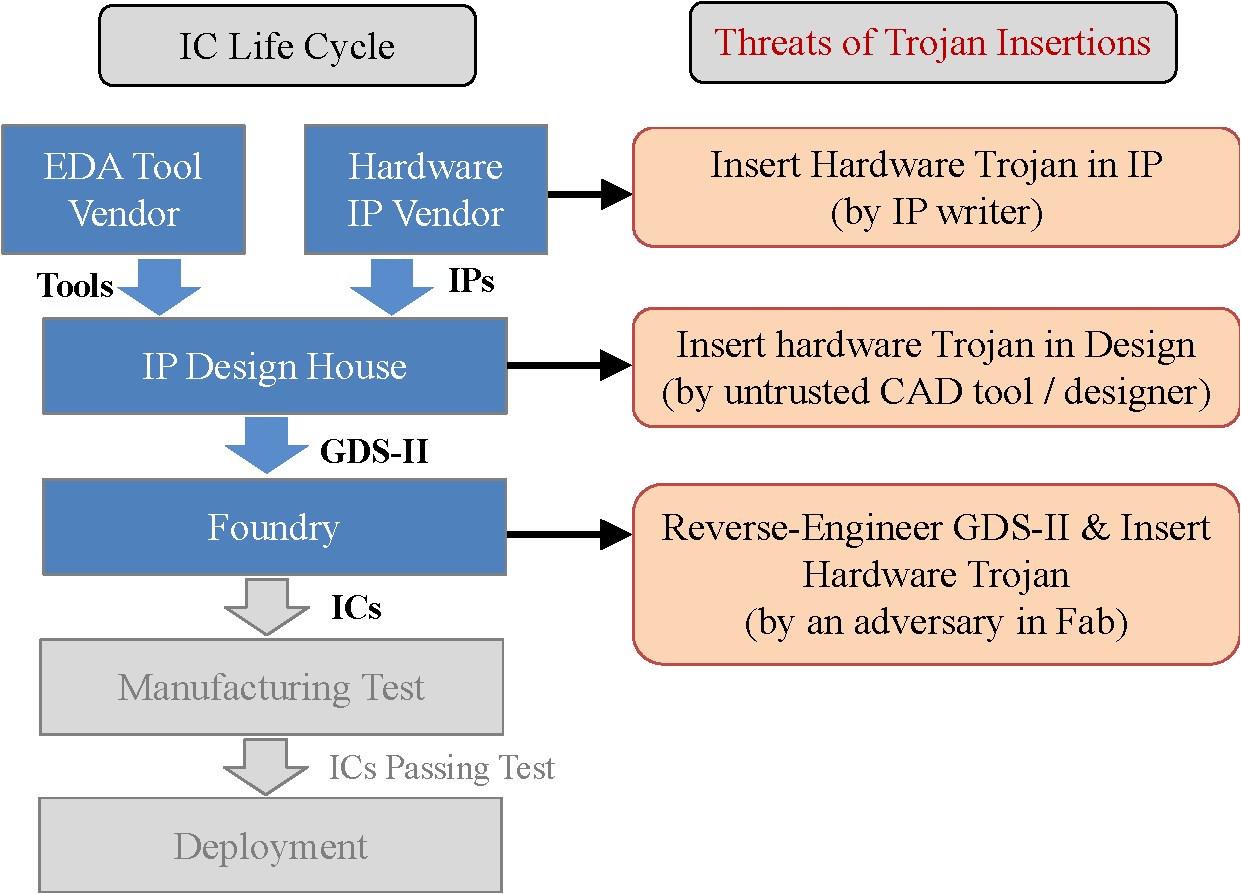
\includegraphics[width=7.8cm]{figure/HT_insert.pdf}
%\caption{Hardware Trojans inserted at different stages \cite{article:SB}.}
%\label{fig:3PIP_threats}
%\end{figure}


%\begin{table*}[!t]
%\renewcommand{\arraystretch}{1.0}
%\caption{Comparison with Related Work}
%\centering
%\begin{tabular}{c|c|c|c|c|c|c}
%\hline
%\hline

%\multicolumn{1}{c|}{\multirow{2}{*}{Technique}}    & Security          &Vulnerability  &\multicolumn{1}{c|}{\multirow{2}{*}{Recovery}}     &\multicolumn{1}{c|}{\multirow{2}{*}{Optimize area}}  & \multicolumn{1}{c|}{\multirow{2}{*}{Optimize delay}}  & Optimize power    \\
%    &constraints    &variation  &   &  &   &or energy   \\
%\hline
%\hline




%\cite{article:JR3}        &Yes      &No   &No     &No   &No    &Yes    \\

%\cite{conference:XC}      &Yes       &No   &Yes    &No   &No    &No    \\

%\cite{article:SR}        &Yes       &No   &No     &Yes   &Loose delay constraints    &Loose power constraints    \\

%\cite{conference:AS}      &Yes      &No   &No     &No   &No    &Yes   \\

%\cite{article:YS}        &Yes       &No   &No     &No   &Loose delay constraints    &Yes   \\



%\cite{article:CL}        &Yes       &No   &No     &No   &Tight delay constraints    &No     \\

%\cite{article:XC}        &Yes       &No   &Yes     &Loose area constraints   &Loose delay constraints    &No     \\


%This study                &Yes       &Yes   &No     &Yes   &Tight delay constraints    &No     \\

%\hline
%\hline
%\end{tabular}
%\label{table:comparison_related_works}
%\end{table*}

%\subsection{Runtime Monitoring}

%Runtime monitoring detects hardware trojans by continuously checking and verifying the behavior of side-channel signals or circuit operations, and recent researchers have focused on improving runtime hardware trojan detection accuracy. He \textit{et al.} \cite{conference:JH} developed a runtime trust evaluation framework based on on-chip electron magnetic sensors and achieved a high hardware trojan detection accuracy. Hou \textit{et al.} \cite{article:YH} guarded the concerned signals and initiated a hardware interrupt request when abnormal toggling events occurred. Kulkarni \textit{et al.} \cite{conference:AK, article:AK} proposed real-time anomaly detection frameworks based on support vector machines and K-nearest neighbors for many-core architecture. Zhao \textit{et al.} \cite{article:HZ} proposed a runtime trojan detection model that applied chaos theory to characterize side-channel parameters. Malekpour \textit{et al.} \cite{conference:AM} focused on mitigating hardware trojans with a permanent impact on the system and successfully detected hardware trojans with a slightly higher area and performance overheads.

%Researchers also observed the significant increment of resources, power and performance caused by runtime monitoring, and many solutions have been proposed to reduce these increments while maintaining high accuracy of trojan detection. Mohd \textit{et al.} \cite{article:BM} developed a low-power, low-energy and trusted design based on a smart runtime monitoring algorithm. Bao \textit{et al.} \cite{article:CB} demonstrated approaches with low hardware resource overhead for runtime trojan detection with thermal sensors. Zhu \textit{et al.} \cite{article:JZ} obtained a high effectiveness in detecting pervasive hardware security issues with little performance loss. Khalid \textit{et al.} \cite{article:FK} proposed a single power-port current acquisition block using current sensors in time-division multiplexing, which increases detection accuracy with a reduced area overhead.% Hussain \textit{et al.} \cite{conference:MH} demonstrated a runtime energy-efficient hardware trojan localization design for network-on-chips, where the authentication was activated only when the hardware trojans were triggered.

%The main advantage of security monitors is the reconfigurability to various checks without the ``golden model", but these checks are simple, and do not cover the entire circuit \cite{article:SB}. Therefore, finding all hidden trojans using security monitors still cannot be guaranteed although many studies have been proposed to improve the detection efficiency.



\subsection{Security Countermeasures}


%hardware security threats can results from unintentional design flaws [1-3], system side effects [4-7], and intended malicious design modifications [8]-[10]. They usually target security assets, such as cryptographic functions, secure architecture,


%It is extremely difficult to detect all hardware trojans in 3PIPs since there is no known golden model for 3PIPs. IP vendors usually provide source code, which may contain trojans, and a trojan can be very well hidden during normal functional operations. Besides, an attacker may distribute few codes to reduce the trojan footprint, and a large industrial-strength IP can include thousands of lines of code.



Numerous and various functional and parametric tests are required to verify whether a 3PIP contains hardware Trojans. However, testing a black-box component is difficult and time-consuming, and it is impractical to perform such an exhaustive test for a large and complex design. Therefore, a number of countermeasures have been developed against hardware Trojans at the design stage \cite{article:WH}. Hardware security primitives provide built-in self-authentication against various threats and vulnerabilities arising at different phases \cite{article:DM}. System and architectural protection techniques prevent information leakage through hardware isolation and build trusted execution environments \cite{article:NH}. Side-channel protection techniques introduce noise or randomization in the software implementation to eliminate side-channel leakage \cite{conference:HK}. IP protection techniques use hardware watermarking or steganography to protect an IP against threats \cite{article:AS1}. Machine learning-assisted designs provide defenses against security threats or enhance system robustness \cite{article:SY1}.

Although hardware Trojan detection methods are implemented in different design stages, finding all hardware Trojans cannot be guaranteed even with the most cutting-edge technologies. However, many applications, such as banking and military systems, have high security requirements \cite{conference:XZ}. Therefore, Trojan-tolerant design methodologies are another way to protect designs from Trojan attacks \cite{article:KX}.


\subsection{Design-for-Trust}



The design-for-trust techniques use strategies at design time to help detect hardware Trojans or mute the attack effects at runtime \cite{article:JR3}. Many studies have attempted to detect malicious outputs by duplicating 3PIPs and to avoid collusion between parent and child tasks from the same vendor. Incorporating the above design constraints (i.e., security constraints) in the MPSoC design process has attracted the attention of researchers.

Reecee \textit{et al.} \cite{article:TR} identified hardware Trojans through comparisons of two similar untrusted designs by testing functional differences for all possible input combinations. Beaumont \textit{et al.} \cite{conference:MB} developed an online Trojan detection architecture that implements fragmentation, replication, and voting. Cui \textit{et al.} \cite{conference:XC} implemented both Trojan detection and fast recovery at runtime for mission-critical applications, using recomputation with IP cores from different vendors. Shatta \textit{et al.} \cite{conference:MS} presented methodologies that detect the errors triggered by hardware Trojans in 3PIPs using voters, and recover the system by replacing the error.









Security constraints, including duplication and 3PIP vendor diversity, have been recently proposed for hardware Trojan protection, and high-level synthesis is the ideal level for incorporating security constraints \cite{conference:JR2}. However, fulfilling the security constraints in task scheduling may results significant overheads in system performance, chip area and power, and researchers have started to reduce these overheads. Rajmohan \textit{et al.} \cite{article:SR} proposed a PSO-based hybrid evolutionary algorithm, and Sengupta \textit{et al.} \cite{conference:AS} proposed a bacterial foraging optimization-based design space exploration method to achieve a task schedule with higher security and less hardware overhead. Sun \textit{et al.} \cite{article:YS} minimized the energy consumption while simultaneously protecting the MPSoC against the effects of hardware Trojans with security constraints. Cui \textit{et al.} \cite{article:XC} solved the online hardware Trojan detection and recovery problem with graph-theory models that minimize the implementation cost of the design budget and area overhead. Liu \textit{et al.}\cite{article:CL} proposed a set of task scheduling methods to reduce the increments of performance and hardware due to security constraints. Wang \textit{et al.} \cite{article:NW, conference:NW} optimized the design budget and system performance with a minimized number of unprotected communications.



The above techniques were developed to optimize design overheads when adopting security constraints, but the optimization space is limited \cite{article:SR, conference:AS, article:YS, article:XC}. Some researchers also treat security constraints as loose constraints (some constraints are not applied to tasks and communications) to achieve tight design targets, but they forget to minimize the induced design's security losses \cite{article:CL, article:NW, conference:NW}, and the induced chip area is also not optimized. Hardware Trojans intend to attack the targets with higher vulnerability to create larger damage to the systems or leakage the confidential information, and the vulnerabilities of tasks or communications can differ by $\times10^3$ times in the same benchmark \cite{conference:HS}. This indicates that the design's performance and area can be further reduced with a small penalty of vulnerability increment by removing some ``proper'' security constraints from tasks and communications. Therefore, we try to minimize both the circuit vulnerability against hardware Trojan attacks and the chip area under the performance constraints in this study.




\section{Preliminaries and Problem Description}

In this section, we present preliminaries and describe the problem considered in this study.


\subsection{Threat Model}



Hardware Trojan attacks are intended to affect normal circuit operation, potentially with catastrophic consequences in critical applications in the domains of banking, space and military \cite{article:SB1}. They can also aim to leak secret information from inside a chip through covert channels or affect the reliability of a circuit through undesired process changes that cause device ware-out and long-term reliability issues \cite{article:RC}. From the perspective of the activation methods, hardware Trojans can be classified as either \textit{always-on} or \textit{conditionally triggered}. An always-on Trojan may be inserted in rarely accessed places and its footprint is kept small. Conditionally triggered Trojans hibernate initially, and are activated either by the Trojan implanter or by on-chip triggers \cite{article:CL}.

In this study, we adopt the same threat model in \cite{article:CL, article:YS}, which primarily focuses on detecting (or mitigating) malicious modifications. The Trojan may cause the task running on the malicious 3PIP to either produce incorrect output or collude with Trojans in another 3PIP core from the same vendor. As a result, the following two cases can occur at runtime: 1) \textit{Malfunction:} due to the insertion of the malicious logic into a 3PIP core, the outputs of the infected cores will be altered at some undetectable points; 2) \textit{Trojan collusion and Trojan triggering between Cores:} Trojans that are distributed on multiple cores to reduce the chance of being detected, and some malicious communication paths can also be established between cores by writing some illegal values to certain secret memory space. Therefore, with these secret communication channels, a malicious logic in one core can trigger the Trojans in another core, and active Trojans in different cores can collude to cause catastrophic consequences to the systems. Examples of the vulnerabilities caused by hardware Trojans in 3PIPs could be: information leakage, control flow violation, fault injection, side-channel leakage, and so on.

In this study, we target embedded platforms which execute application-specific tasks and have high security requirements, and such platforms are widely-used in auto-motive, safety-critical systems, etc \cite{article:YS}. The SoC used in these systems are vulnerable to various Trojans attacks when the untrusted 3PIPs get integrated into this SoC. Because the hardware Trojans in 3PIPs could be passed down the design cycle to post-silicon and all the fabricated chips contain such hardware Trojans. In such security-critical systems, designers always have prior knowledge of the application and its runtime constraints, and they can decide to purchase 3PIPs from different vendors, and bind tasks to IP cores.

\subsection{Security Constraints}

It is impossible to detect all hardware Trojans in 3PIPs even with the most advanced techniques, and therefore, runtime validation approaches provide a last line of defense against  potentially undetected Trojans \cite{article:SB}. Integrating security constraints in the task scheduling process enables the runtime validation using untrusted 3PIPs, and the effectiveness of the security constraints in detecting the deliberate faults caused by Trojans and isolating the triggered Trojans are explained in \cite{article:JR3}. The two types of security constraints which are also introduced in \cite{conference:JR2, article:SR, conference:AS, article:YS, article:XC, article:CL, article:NW, conference:NW} handle two major types of Trojans: Those tampering program outputs and those leaking information through undesired communications. These security constraints are described as follows.% tasks are scheduled under the following two types of security constraints. %\cite{conference:JR2, article:SR, conference:AS, article:YS, article:XC, article:CL, article:NW, conference:NW}.%: \textit{task duplication} and \textit{vendor diversity}.


\subsubsection{Duplication-With-Diversity}

To detect hardware Trojans, each task is executed in duplicate on the cores from different vendors, and the outputs of these cores are compared by a trusted component (not designed by the third party). This type of security constraints is applied to tasks, and ensures the trustworthiness of task outputs \cite{conference:DG}.

Duplication-with-diversity is set based on the fact that the probability of Trojans implanted by different attackers having the same trigger input is quite low, and it is virtually impossible that two cores from different IP vendors will output the same tampered results after the same trigger input \cite{article:NV}.% In the following descriptions, the duplicated task of $v_i$ is denoted as $v_{i'}$.




\subsubsection{Isolation-With-Diversity}

To mute undesired and potentially malicious communication paths and at the same time isolate a Trojan from the rest of the system, data-dependent tasks are executed on the cores fabricated from different IP vendors. This type of security constraint is applied to the communications between tasks, which ensures that all the valid communication paths are between 3PIPs from different vendors.

%This type of security constraint can be used to isolate the triggered hardware Trojans. Because attackers always distribute Trojans in multiple IP cores and construct secret communications between IP cores to leak information or to trigger the hibernating Trojans, and these secret communications between IP cores from the same vendor cannot be acquired by other vendors \cite{article:JR3}.

To mute Trojan footprints, attackers may distribute Trojans in multiple IP cores and construct secret communication paths between IP cores to leak information or to trigger the hibernating Trojans. These secret communication paths between IP cores from the same vendor cannot be acquired by other vendors \cite{article:JR3}. Although redundant execution approaches, including voting architecture \cite{conference:MB}, dual/triple modular redundancy \cite{conference:DG}, and duplication-with-diversity, can detect hardware Trojans by comparing the outputs of cores from different vendors with the same input, they cannot cut off secret communications between multiple IP cores. Therefore, this isolation-with-diversity is also introduced to isolate the triggered hardware Trojans from the rest of the system.





%Analyzing a circuit's vulnerability against hardware Trojan attacks at different levels is a key step towards trusted design development, because sections of a circuit with low controllability and observability are considered potential areas for implementing hardware Trojans \cite{article:MT, article:JC,article:YD}. The vulnerability analysis at behavioral level quantifies the difficulty of activating each line of a code and observing internal signals and and primary inputs through outputs. This analysis consists of \textit{statement analysis} which measures the statement execution conditions, and \textit{observerability analysis} which evaluates reachability of signals and observability through circuit primary output \cite{conference:HS}. Hardware Trojans may choose the target with low observability and high statement hardness.% and the experimental results in \cite{conference:HS} reveal that the vulnerabilities of tasks or communications can differ by $\times10^3$ times in the same benchmark.

%\textcolor{red}{Salmani et al. \cite{conference:HS} introduced a method for analyzing hardware description languages at the behavioral level. This approach entails analyzing data and control flows at the behavioral level to determine the execution hardness of each statement and the observability of internal signals. Such analysis aids in assessing the detectability of Trojan insertions across various sections of the code.}



%Thus the vendor diversity constraint which forces the is also introduced to isolate the triggered hardware Trojans from the rest of the system.

%To mute the Trojan footprint, the attacker always distributes Trojans in multiple IP cores and constructs secret communications between cores to leak information or to trigger the hibernating Trojans. In this study, we assume that the secret communication between cores from the same vendor cannot be acquired by other vendors and that the attackers of different vendors plant different hardware Trojans.

%In a task graph with $n$ nodes and $m$ edges, the number of task duplication constraints is $n$, and the number of vendor diversity constraints is $2m$ (both the task graph and the duplicated task graph contain $m$ vendor diversity constraints). Therefore, the number of all security constraints (denoted as $scy$) is $n+2m$.


\begin{figure}[!t]
\centering
\hspace*{-0.8em}
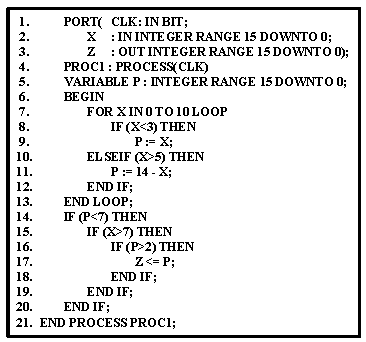
\includegraphics[width=8cm]{figure/sample_code.pdf}
\caption{Example of code for vulnerability analysis.}
\label{fig:sample_code}
\end{figure}




\begin{figure}[!t]
\centering
\begin{tabular}{c}
%\hspace{-1em}
\subfigure [] {
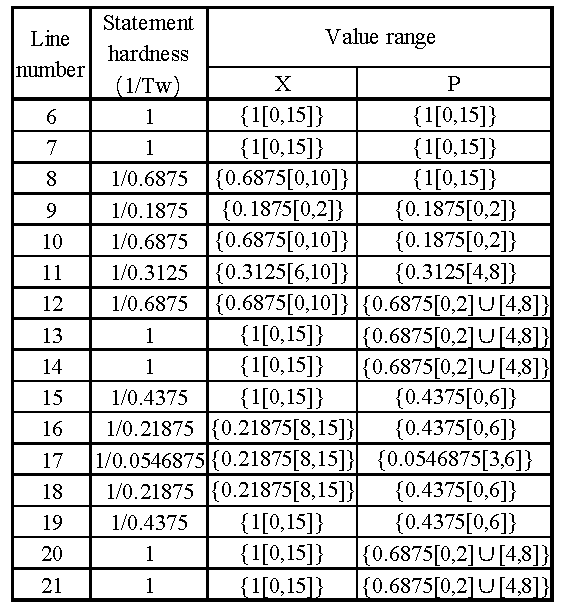
\includegraphics[width=7.6cm]{figure/statement_hardness_and_variable_ranges.pdf}\label{subfig:statement_hardness_and_variable_ranges}
}
\\
\hspace{-7em}


  \begin{minipage}{0.13\textwidth}
    \centering
    \subfigure[]{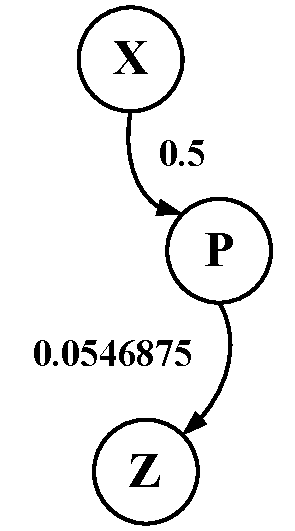
\includegraphics[width=1.5cm]{figure/data_flow_graph.pdf}\label{subfig:data_flow_graph}}
  \end{minipage}

  \begin{minipage}{0.23\textwidth}
    \centering
    \subfigure [] {
    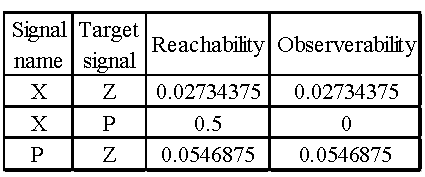
\includegraphics[width=5.6cm]{figure/observability_of_signals.pdf}\label{subfig:observability_of_signals}}
    \end{minipage}

\end{tabular}
\caption{Example of vulnerability analysis. \subref{subfig:statement_hardness_and_variable_ranges} Statement hardness of signals.  \subref{subfig:observability_of_signals} Observability of signals. \subref{subfig:data_flow_graph} Data flow graph.}
\label{fig:vul_analysis}
\end{figure}

\subsection{Vulnerability Analysis}

Analyzing a circuit's vulnerability against hardware Trojan attacks at different levels is a key step towards trusted design, because sections of a circuit with low controllability and observability are considered potential areas for hardware Trojans insertions \cite{article:MT, article:JC,article:YD}. The vulnerability analysis at behavioral level consists of \textit{statement analysis} and \textit{observerability analysis}, which quantifies the difficulty of activating each line of a code and observing internal signals \cite{conference:HS}. The vulnerabilities of different signals vary a lot, and hardware Trojans may choose the target with low observability and high statement hardness to attack.

Adopted from the work presented in \cite{conference:HS}, an example of vulnerability analysis of a small behavior code (see Fig. \ref{fig:sample_code}) is also presented in Fig. \ref{fig:vul_analysis}. The \textit{statement analysis} first measures the statement execution conditions. The notation $W[L,U]$ is developed for each signal where $W$ represents the weight of the value range, and $L$ and $U$ show the lower and upper limits of the value range. The weight of a range is defined as $\frac{U-L+1}{U_O-L_O+1}$, where $U_O$ and $L_O$ are the declared upper and lower limits of the controlling signals. Because the hardware Trojans are always designed with small triggering probability to escape from the Trojan detection methods, and the \textit{statement hardness} is defined as $1/W$. Fig. \ref{subfig:statement_hardness_and_variable_ranges} gives the statement hardness of the signals $X$ and $P$.

The \textit{observerability analysis} evaluates reachability of signals and observability through circuit primary output, because a behavioral-level Trojan usually targets a signal with low observability to carry out an attack. A weight data graph of signals is constructed in Fig. \ref{subfig:data_flow_graph}, where the nodes are circuit signals and the directed edges are their dependency. For example, the signal $X$ appears in Lines 8 and 11 where the target signal is $P$. The reachability of edge $(X,P)$ is $0.1875+0.3125=0.5$, where 0.1875 and 0.3125 are shown in Fig. \ref{subfig:statement_hardness_and_variable_ranges}, but the observability of this edge is 0 as the signal $P$ is not an output signal. The reachability and observability of each edge is presented in Fig. \ref{subfig:observability_of_signals}.

%To assess the vulnerability of circuits, we adopt this method. We illustrate this method using a simple example. Fig. \ref{fig:sample_code} displays the sample code, with statement hardness determined by the ratio of execution control signal range to declared range. For instance, if line 7 confines X to 0-10 while its declared range is 0-15, the hardness for line 8, controlled by X, is 11/16=0.6875. Multiple signals multiply their weights for statement hardness. Fig. \ref{fig:statement_hardness_and_variable_ranges} details statement hardness and variable ranges. Fig. \ref{fig:contol_flow_stack} shows control flow stacks. Fig. \ref{fig:data_flow_graph} exhibits the data flow graph, with node denoting signals and directed edges denoting dependencies and weights denoting the sum of weights of corresponding assignment statement. Fig. \ref{fig:observability_of_signals} assesses observability of signals from output Z; internal signal P's influence by X yields 0 observability. Statement vulnerability equals weight multiplied by target signal's observability to output.








\subsection{Motivations}


\begin{figure*}[!t]
\centering
\begin{tabular}{ccc}
\hspace*{-1.5em}
\subfigure [] {
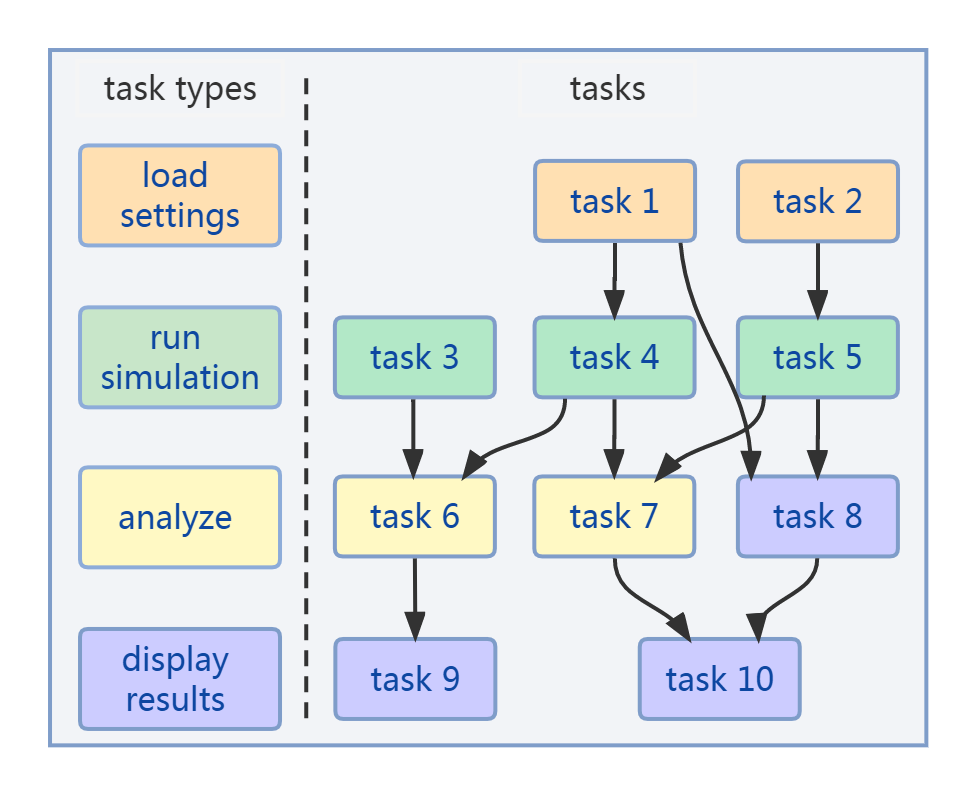
\includegraphics[width=6cm]{figure/tg.png}\label{subfig:tg4}
} &\hspace*{-1.0em}
\subfigure [] {
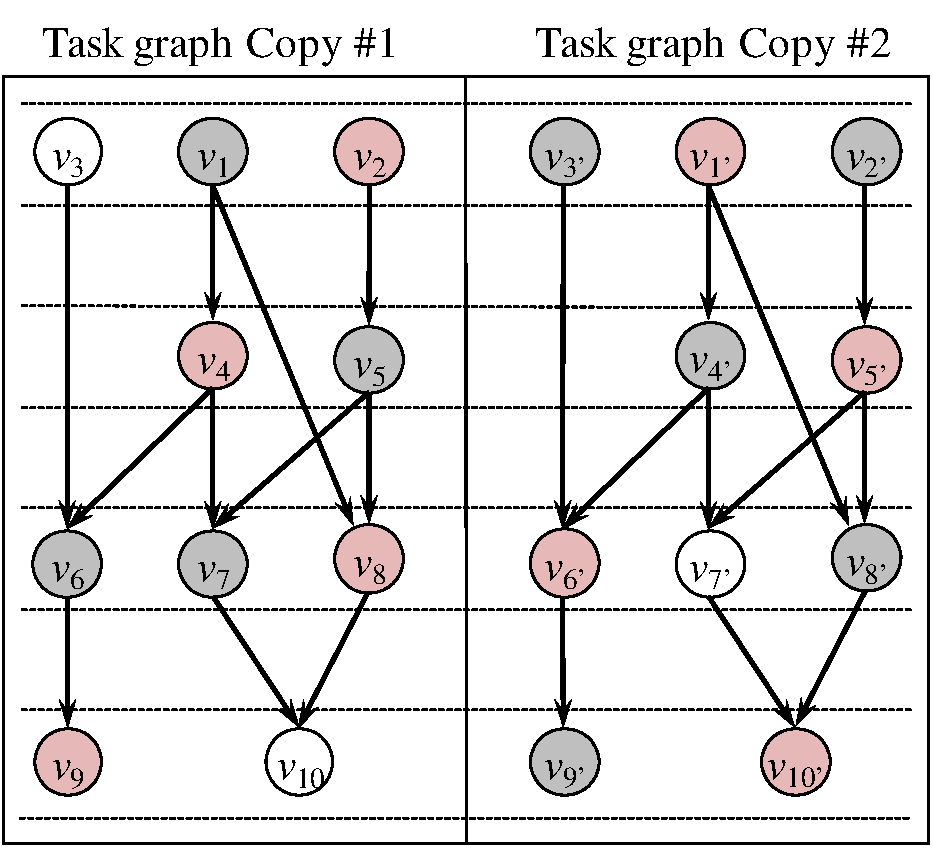
\includegraphics[width=5.45cm]{figure/constraint_example1.pdf}\label{subfig:asap_schedule_security}
} & \hspace*{-0.5em}
\subfigure [] {
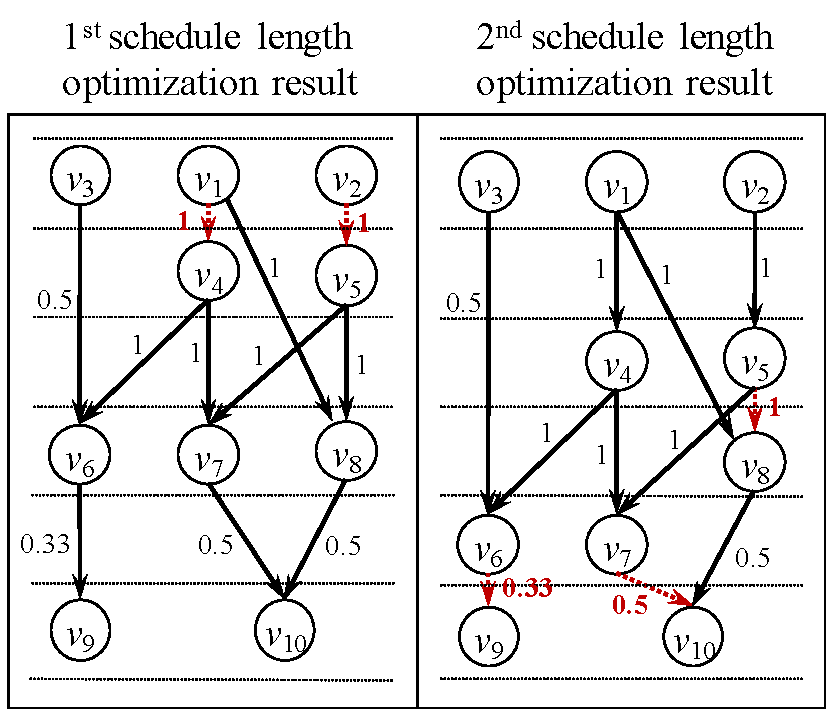
\includegraphics[width=5.75cm]{figure/performance-motivation1.pdf}\label{subfig:performance-motivation}
}
\end{tabular}
\caption{Example of task graph and its schedules. \subref{subfig:tg4} Task graph. \subref{subfig:asap_schedule_security} ASAP schedule with security constraints. \subref{subfig:performance-motivation} Schedule length optimization results.}
\label{fig:security}
\end{figure*}





Fulfilling security constraints may incur significant overheads of performance and area, and Fig. \ref{fig:security} shows an example, where 10 tasks are sorted into 4 different types. All intra-core communication delays are ignored, and the computational times of all tasks are assumed to be 1 unit of time (\textit{ut}), which also equals their inter-core communication delays. Fig. \ref{subfig:tg4} and Fig. \ref{subfig:asap_schedule_security} show the task graph and its as-soon-as-possible (ASAP) task schedule with security constraints, where tasks colored white, gray, and pink are assigned to the 1st, 2nd, and 3rd vendors, respectively. The duplicated task of $v_i$ is denoted as $v_{i'}$. Satisfying all security constraints makes the schedule length 7 \textit{ut}, and 6 cores from 3 IP vendors are required.

%Researchers have started to explore the possibility of grouping data-dependent tasks into a cluster to reduce the number of IP vendors required \cite{article:XC, article:CL, article:NW} or the system performance \cite{article:CL, article:NW, conference:NW}, which violates the vender diversity constraints. However, a pre-defined maximum permissible security loss is allowed to reduce the overheads of power, area, energy, and performance \cite{article:SR}, so designers also seek the solutions to minimize system security loss with the desired targets.


\subsubsection{Vulnerability Increment in Performance Optimization}

To reduce the performance overhead, researchers have imposed loose security constraints during task scheduling and explored the possibility of assigning data-dependent tasks into a single core to hide the inter-core communication delay \cite{article:CL, article:NW, conference:NW}. In this study, clustering the connected data-dependent tasks into one core is denoted as \textbf{edge contraction}, and the edge that represents an intra-core communication is a \textbf{contracted edge}.

Edge contraction leaves the corresponding communication without protection, and this communication is vulnerable to hardware Trojans. Traditional methods that optimize system performance either ignore the consequence security loss \cite{article:CL} or treat every communication with the same security importance \cite{article:NW, conference:NW}. However, communications have different vulnerabilities against hardware Trojan attacks, and the vulnerabilities can differ by $\times10^3$ times in the same benchmark \cite{conference:HS}.

The example in Fig. \ref{subfig:performance-motivation} shows the necessity of optimizing the system performance with the consideration of vulnerability variation, where the target is to reduce the schedule length in Fig. \ref{subfig:asap_schedule_security} to 6 \textit{ut}. Traditional methods \cite{article:NW, conference:NW} contract the fewest edges, which are $e_{1,4}$ and $e_{2,5}$ (see the 1st schedule length optimization result in Fig. \ref{subfig:performance-motivation}). However, $e_{5,8}$, $e_{6,9}$, and $e_{7,10}$ might be less vulnerable to hardware Trojan attacks if compared to $e_{1,4}$ and $e_{2,5}$, and contracting these edges causes less vulnerability (see the 2nd schedule length optimization result in Fig. \ref{subfig:performance-motivation}), even though this contracts more edges.





\begin{figure}[!t]
\centering
\begin{tabular}{c}
%\hspace{-1em}
\subfigure [] {
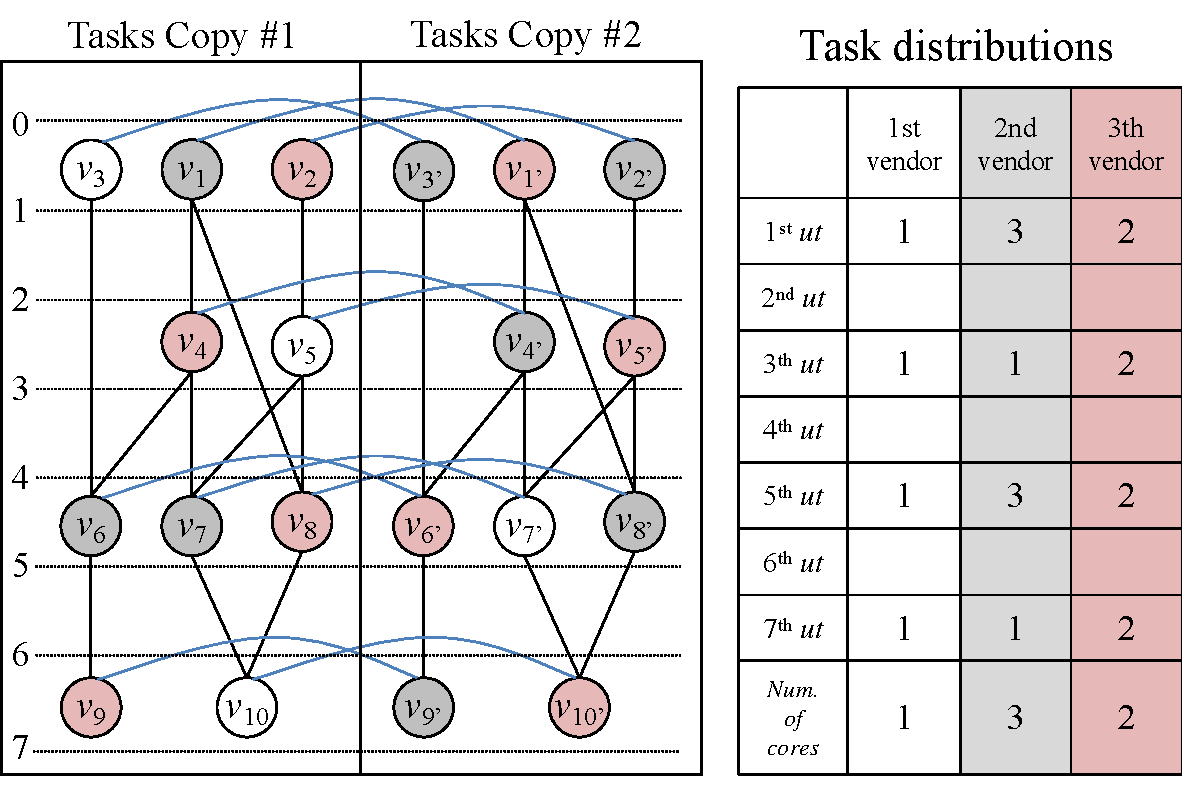
\includegraphics[width=7.4cm]{figure/security1.pdf}\label{subfig:resource_req1}
} \\
%\hspace{-1em}
\subfigure [] {
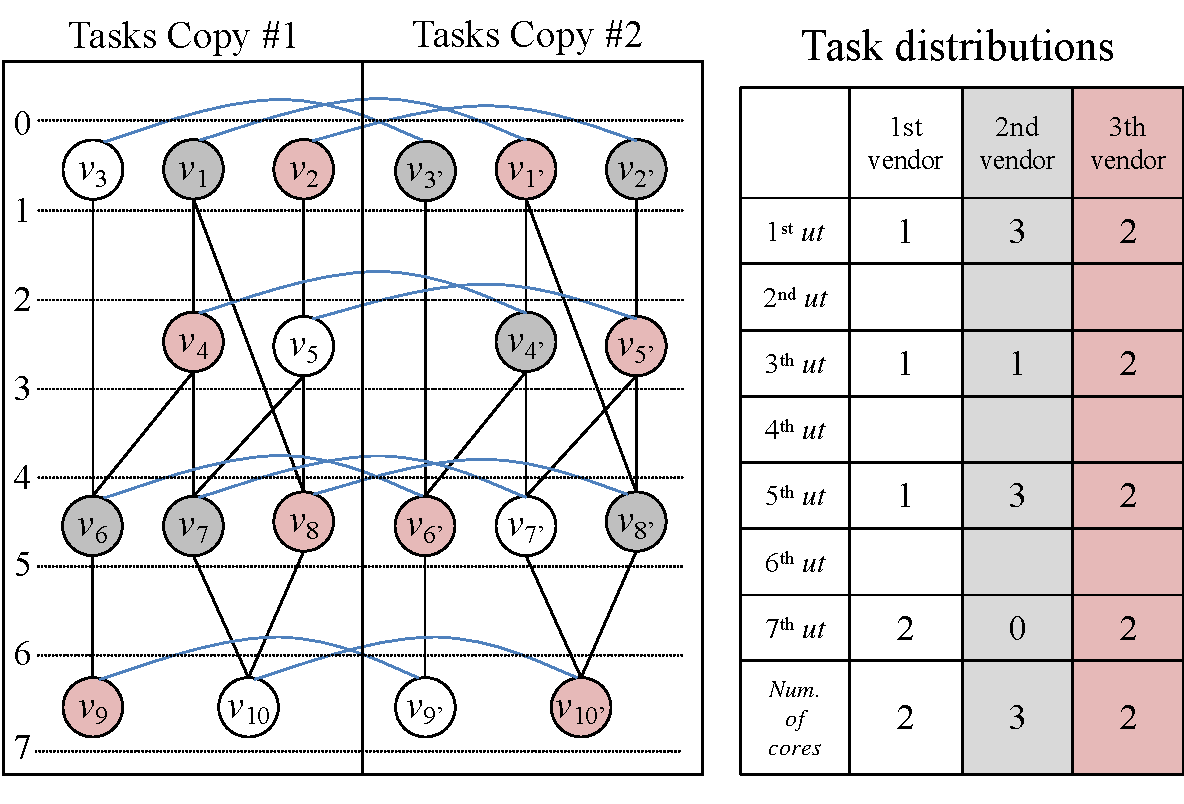
\includegraphics[width=7.4cm]{figure/security2.pdf}\label{subfig:resource_req2}
}
\end{tabular}
\caption{Example of vendor assignments. \subref{subfig:resource_req1} Vendor assignment and its ASAP schedule, which requires 6 cores. \subref{subfig:resource_req2} Vendor assignment and its ASAP schedule, which requires 7 cores.}
\label{fig:resource_req_motivation}
\end{figure}





\subsubsection{Reducing Cores in Vender Assignment}

In the vendor assignment stage, all tasks are partitioned into many groups such that all tasks in a group are executed by the cores from the same vendor. Traditional methods start to optimize the number of cores after the vendor assignment stage when the number of cores required can be evaluated \cite{article:YS, article:XC, article:CL, article:NW}. However, the vendor assignment results also determine the number of cores required, and the example in Fig. \ref{fig:resource_req_motivation} explains the reason. In this example, the performance constraint is assumed to be 7 $ut$, and all security constraints are satisfied, which are represented by the blue (\textit{duplication-with-diversity}) and black (\textit{isolation-with-diversity}) lines between tasks. Fig. \ref{subfig:resource_req1} and Fig. \ref{subfig:resource_req2} give two different vendor assignments and their ASAP schedules. With the vendor assignment given in Fig. \ref{subfig:resource_req1}, the scheduling result requires 6 cores, but 7 cores are required with the vendor assignment shown in Fig. \ref{subfig:resource_req2}.






\subsection{Problem Description}

Clustering data-dependent tasks to reduce schedule length violates \textit{isolation-with-diversity}, leaving the corresponding intra-core communications unprotected. Although incorporating security constraints in the design process cannot guarantee a full protection from all hardware Trojan attacks, the vulnerability against hardware Trojan attacks can be significantly reduced. In this study, the vulnerability of a communication is regarded as the reduced vulnerability after applying security constraints to this communication, and the vulnerability analysis \cite{conference:HS} can be performed before our method to first determine the vulnerabilities of communications. The problem considered in this study can be described as follows.

\begin{problem}
The inputs of this problem are the task graph $TG$, vendor and performance constraints, core speeds of vendors, and vulnerability of each communication. The target is to find a schedule with the lowest design's vulnerability against hardware Trojan attacks, and the number of cores required is also optimized.
\end{problem}


The design's vulnerability $vul_s$ is regarded as the accumulated vulnerabilities of all unprotected communications, which can be calculated as follows:
\begin{equation}
vul_s=\sum \limits_{e\in E_c}vul(e)
\end{equation}

\noindent where $E_c$ is the set of all unprotected communications, and $vul(e)$ is the vulnerability of $e$.% The notations used in this paper are also shown in Table \ref{table:notation}.

%\begin{table}[!h]
%\renewcommand{\arraystretch}{1.06}
%\caption{Descriptions of Notations}
%\centering
%\begin{tabular}{l|p{6cm}}
%\hline
%\hline

%Notation    &Description     \\
%\hline
%\hline

%$v_i$   &The $i$-th task, and its duplicated task is $v_{i'}$.\\

%$c$   &The cluster, which consists of a set of tasks.\\

%$e_{ij}$  &The communication from task $v_i$ to task $v_j$. \\

%$vul(e)$   &The vulnerability of $e$.\\

%$vul_s$   &The design's vulnerability of a schedule.     \\

%$dly(e)$   &Inter-core communication delay of $e$.  \\

%$w(e)$   &Evaluated weight of contracting $e$.   \\

%$prob(v_i,t_j)$   &The probability that task $v_i$ is executed in time $t_j$.   \\

%$DG(c,t_j)$   &The number of tasks in cluster $c$ that are executed in time period $t_j$.   \\

%$DG_{max}(c)$   &The maximum of all $DG(c,t_j)$, which estimates the number of cores required for cluster $c$. \\

%$Merge(c_i,c_j)$   &The number of cores reduced after merging clusters $c_i$ and $c_j$.   \\

%\hline
%\hline
%\end{tabular}
%\label{table:notation}
%\end{table}




%In this work, the calculation of $risk(e)$ is determined by system designers. All possible reasons for the Trojan attack via $e$ should be considered, such as the types of connected tasks, the importance of information transmitted, and the difficulty of leaking information.

%To simplify the experiments, the core speeds of all vendors are assumed to be the same. If the core speeds of different vendors vary, this proposed method can easily be extended to fit.





\section{Security-Driven Task Scheduling with Performance Constraints}

In this section, a three-step task scheduling method is proposed, and both the design's vulnerability and the number of cores required are optimized under performance constraints. The three steps of the proposed method are performance-constrained task clustering, vendor assignment with core minimization, and task scheduling.




\subsection{Performance-Constrained Task Clustering}
%System performance is one of the key considerations for designers, and they always put several timing-critical tasks into the same core to change the inter-core communication delays into a much smaller intra-core communication delay to reduce the schedule length \cite{article:CL, article:NW, conference:NW}. However, this brings consequence security loss to the system, which must be optimized under performance constraints.

In this stage, we first apply security constraints to all tasks and communications, and then iteratively assign data-dependent tasks into the same core to meet the performance constraints with the design's vulnerability optimized. Typically, the cores produced by different vendors have different speeds, and the exact speed of each core is not yet determined; thus, we assume that tasks are performed with the slowest speed when optimizing the schedule length. In addition, we discuss only the method of contracting edges in $TG$, and schedule length optimization of the duplicated task graph $TG'$ can be performed in the same manner.

Source and sink nodes $s$ and $t$ are added to $TG$, and directed edges that point from $s$ to 0-indegree nodes and from 0-outdegree nodes to $t$ are also added. An example of the task graph from Fig. \ref{subfig:tg4} with $s$ and $t$ added is given in Fig. \ref{subfig:TG1}. The \textbf{timing violated graph} ($TVG=(V_T, E_T)$) is then constructed by all paths from $s$ to $t$ whose lengths exceed the performance constraints, and it is an induced subgraph of $TG$. $V_T$ consists of $s$, $t$ and all tasks with negative slacks, and $E_T=\{(v_i,v_j)\in E, v_i\in V_T \textrm{~and~} v_j\in V_T\}$. Let $slack(v)$ be the slack time of $v$ under the performance constraint, which is calculated as follows:
\begin{equation}
slack(v) = t_{alap}(v)-t_{asap}(v)-exec(v)
\end{equation}

\noindent where $exec(v)$ is the execution time of task $v$, and $t_{asap}(v)$ and $t_{alap}(v)$ are the ASAP and as-late-as-possible (ALAP) schedules, respectively. Fig. \ref{subfig:tvg1-1} shows an example of $TVG$, where the performance constraint is 5 $ut$ and the delay is 1 $ut$ for each edge.





\begin{figure}[!t]
\centering
\begin{tabular}{ccc}
\hspace*{-1em}
\subfigure [] {
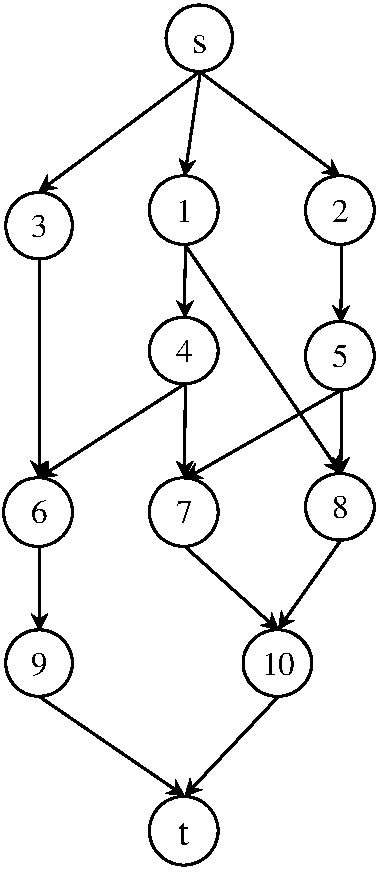
\includegraphics[width=2.3cm]{figure/TG1.pdf}\label{subfig:TG1}
}&\hspace*{-1.6em}
\subfigure [] {
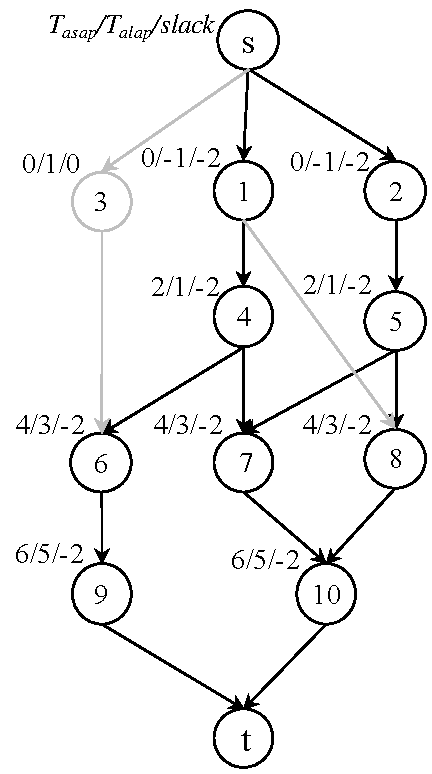
\includegraphics[width=3cm]{figure/tvg.pdf}\label{subfig:tvg1-1}
} &\hspace*{-1.6em}
\subfigure [] {
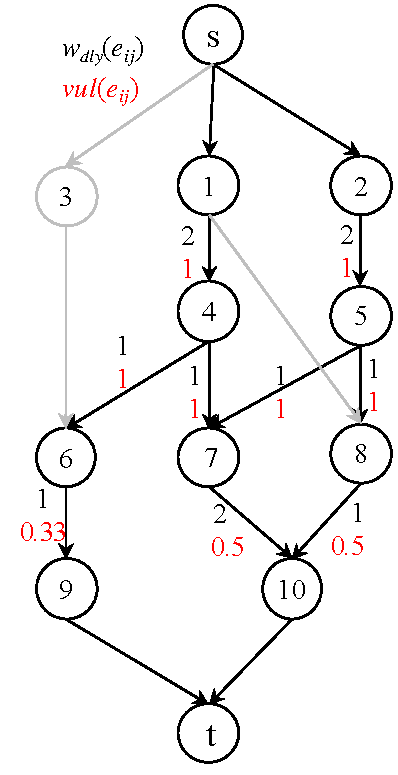
\includegraphics[width=3.05cm]{figure/tvg1.pdf}\label{subfig:tvg1-2}
}
\end{tabular}
\caption{Example of evaluating the timing violated graph. \subref{subfig:TG1} Task graph with $s$ and $t$. \subref{subfig:tvg1-1} $TVG$ with a timing constraint of 5 $ut$. \subref{subfig:tvg1-2} The evaluation of $w_{dly}(e)$.}
\label{fig:weight_e}
\end{figure}

For application-specific IPs, data-dependent tasks might have to be executed by different IP cores, resulting in the corresponding edge being unable to be contracted. Therefore, we only focus on the edges that can be contracted to reduce the schedule length. In the following discussion, we assume that all edges can be contracted for simplicity.

Let $dly(e_{ij})$ be the inter-core communication delay of $e_{ij}$, and all intra-core communication delays are ignored in this study. Contracting an edge ($e_{ij}$) reduces the lengths of all paths that pass through $e_{ij}$ by $dly(e_{ij})$. Let $w_{dly}(e_{ij})$ be the sum of the reduced schedule lengths of all paths (from $s$ to $t$) in $TVG$ after contracting $e_{ij}$, and it is calculated by the following equation:
\begin{equation}
w_{dly}(e_{ij})=path_{tvg}(e_{ij})*dly(e_{ij})
\end{equation}


\noindent where $path_{tvg}(e_{ij})$ is the number of paths in $TVG$ that pass through $e_{ij}$.



Fig. \ref{subfig:tvg1-2} illustrates the $w_{dly}(e_{ij})$ and $vul(e_{ij})$ of all edges in $TVG$, which are indicated next to the edges. The target in the schedule length optimization stage is to contract the edges with larger schedule length reduction $w_{dly}(e_{ij})$ and smaller vulnerability $vul(e_{ij})$. Therefore, the total weight that evaluates an edge $e_{ij}$ contraction, denoted as $w(e_{ij})$, can be calculated as follows:
\begin{equation}
w(e_{ij}) = \frac{w_{dly}(e_{ij})}{vul(e_{ij})}
\label{equ:weight_e}
\end{equation}

%Fig. \ref{subfig:tvg1-2} illustrates the $w_{dly}(e_{ij})$ and $risk(e_{ij})$ in $TVG$, which are indicated next to the edges.%, and the $dly(e)$ of all edges is 1 $u.t.$.% Choosing the edges with larger $w(e_{ij})$ indicates that less edges will be contracted until the performance constraint is reached.


However, not all edges can be contracted with respect to multicore parallel execution. Let $in\_edge(v)$ be the set of edges that end with $v$, and let $out\_edge(v)$ be the set of edges that start from $v$. Edges in $TG$ that belong to the same $in\_edge(v)$ or $out\_edge(v)$ are called \textbf{brother edges}. If an edge is contracted during performance optimization, all its brother edges can no longer be contracted. The reason is that contracting brother edges means the tasks that once could be executed parallel in different cores now must be executed sequentially in the same core, and this may result in an increased schedule length. For example, contracting brother edges $e_{4,6}$ and $e_{4,7}$ in Fig. \ref{subfig:tvg1-1} makes $v_6$ and $v_7$ need to be conducted sequentially in the same core, but they can be computed once concurrently in different cores.

In addition, two edges belonging to the same path in the $TVG$ should not be contracted simultaneously, and this avoids the over-optimization of the path length, which causes additional vulnerability against hardware Trojan attacks. The following example explains the reason, where the edges $e_{1,4}$ and $e_{4,7}$ belong to the same path in $TVG$ (refer to Fig. \ref{subfig:tvg1-1}). Suppose that contracting either $e_{1,4}$ or $e_{4,7}$ will make the path length smaller than the performance constraint, and contracting $e_{1,4}$ and $e_{4,7}$ at the same time causes additional vulnerability.


Then, a weighted \textbf{edge contraction conflict graph} ($ECCG=(V_E,E_E)$) is constructed to represent whether every pair of edges in $TVG$ can be contracted simultaneously. Each vertex in $V_E$ represents an edge in $TVG$ that can be contracted, and the weight of a vertex in $V_E$ equals the weight of the corresponding edge in $TVG$. Two vertices in $V_E$ are connected when their corresponding edges cannot be contracted simultaneously, under one of the following two situations:
\begin{enumerate}
\item These two edges are brother edges (with respect to the multicore parallel execution);
\item These two edges belong to the same path in $TVG$ (to prevent the over-optimization of the path length).
\end{enumerate}




\begin{algorithm}[!t]
\caption{Task clustering with performance constraint, $task\_cluster(TG, pc)$.}
\label{alg:PCTC}
\begin{flushleft}
{\textbf{Input:}}
task graph, $TG$;\\
\hspace*{2.8em}performance constraint, $pc$.\\
{\textbf{Output:}} performance-constrained clustering result, $TC$.
\end{flushleft}
\begin{algorithmic}[1]
\WHILE{$TG.schedule\_length > pc$}
\STATE Construct $TVG$ from $TG$.
\FOR{each $e$ in $TVG$}
\STATE Calculate $w(e)$;
\ENDFOR
\STATE Construct $ECCG$ from $TVG$;
\FOR{Each node $e$ in $ECCG$}
\STATE $ECCG.node\_weight(e)=w(e)$;
\ENDFOR
\STATE Calculate $MWIS$ in $ECCG$;
\FOR{each node $e$ in $MWIS$}
    \STATE Contract the corresponding edge $e$ in $TG$;
\ENDFOR
\ENDWHILE
\end{algorithmic}
\end{algorithm}

The maximum weight independent set (MWIS) of $ECCG$ is calculated by the method proposed in \cite{conference:LC}, and the target is to find a set of edges with maximum weight that can be contracted simultaneously. Algorithm \ref{alg:PCTC} shows details of the performance-constrained task clustering algorithm with the goal of minimizing the design's vulnerability. In the first step (\textit{Lines 2-5}), $TVG$ is constructed from $TG$, and the weights of all edges in $TVG$ are evaluated. In the second step (\textit{Lines 6-10}), the weighted $ECCG$ is built, and its MWIS is calculated. In the third step (\textit{Lines 11-13}), the MWIS-selected edges in $TG$ are contracted. These steps are iteratively repeated until the performance constraint is satisfied.


\begin{figure}[!t]
\centering
\begin{tabular}{ccc}
\hspace*{-1.0em}
\subfigure [] {
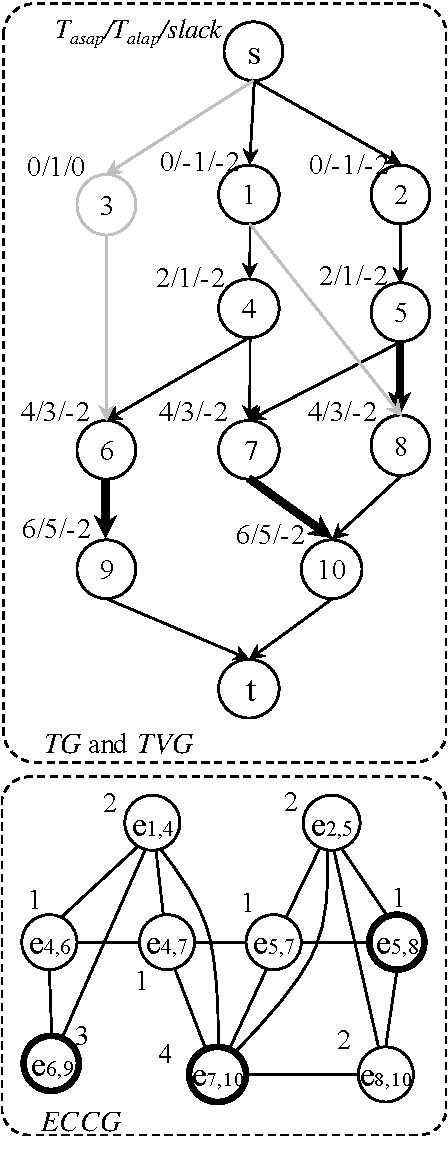
\includegraphics[width=2.8cm]{figure/EVG1.pdf}\label{subfig:EVG1}
} &\hspace*{-1.7em}
\subfigure [] {
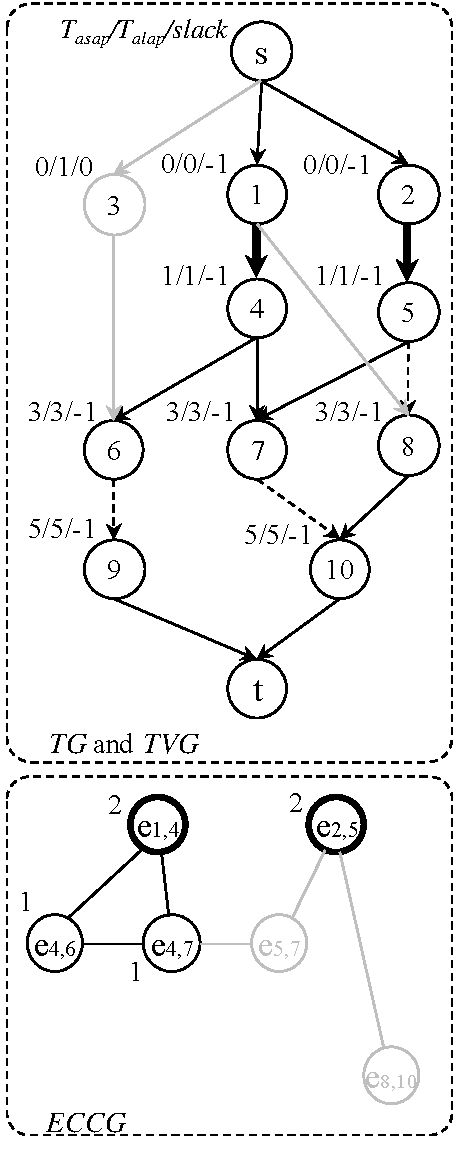
\includegraphics[width=2.8cm]{figure/EVG2.pdf}\label{subfig:EVG2}
} &\hspace*{-1.7em}
\subfigure [] {
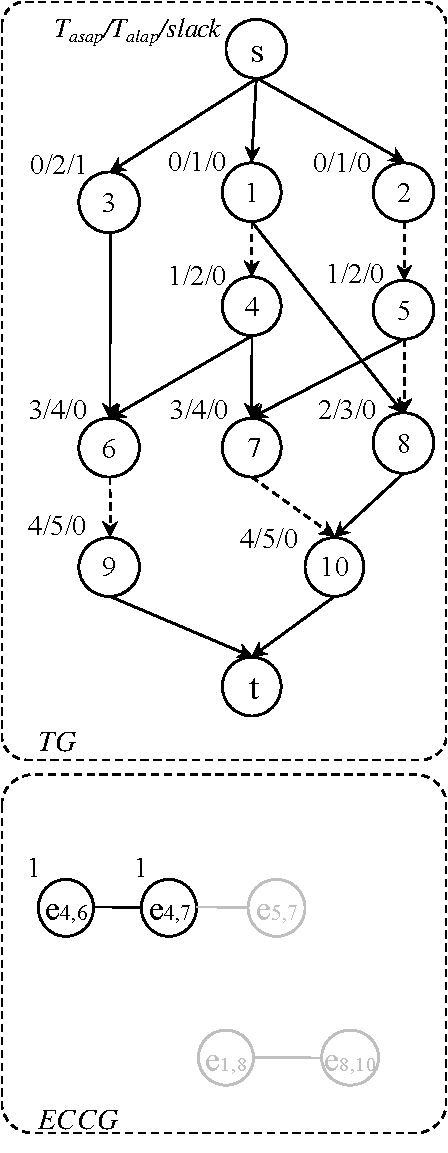
\includegraphics[width=2.8cm]{figure/EVG3.pdf}\label{subfig:EVG3}
}
\end{tabular}
\caption{Example of performance-constrained task clustering procedure. \subref{subfig:EVG1} $TVG$ and its corresponding $ECCG$ before task clustering. \subref{subfig:EVG2} $TVG$ and its corresponding $ECCG$ after 1st iteration of task clustering. \subref{subfig:EVG3} $TVG$ and corresponding $VCG$ after 2nd iteration of task clustering.}
\label{fig:TC}
\end{figure}


With the vulnerabilities of communications given in Fig. \ref{subfig:tvg1-2}, an example of performance-constrained task clustering is shown in Fig. \ref{fig:TC}, where we are about to optimize the schedule length by 2 $ut$. The $TVG$ consists of the nodes and edges with black color, and dashed lines are the contracted edges. $ECCG$ is given beneath the corresponding $TVG$, and the weight of contracting an edge is marked next to the node in $ECCG$. $TVG$ and its corresponding $ECCG$ are constructed (see Fig. \ref{subfig:EVG1}), and its MWIS is $\{e_{5,8}, e_{6,9}, e_{7,10}\}$ which is contracted in the first iteration. Then, both $TVG$ and $ECCG$ are updated as shown in Fig. \ref{subfig:EVG2}, where $e_{5,7}$ and $e_{8,10}$ are not in $ECCG$ because their brother edges $e_{5,8}$ and $e_{7,10}$ are already contracted. The MWIS of the current $ECCG$ is $\{e_{1,4}, e_{2,5}\}$, and after contracting these edges, Fig. \ref{subfig:EVG3} yields the final clustering results, with the performance constraint satisfied.% and the corresponding $ECCG$, and $e_{5,8}$ is contracted in the final iteration.



\subsection{Vendor Assignment with Core Minimization}

%With performance-constrained task clustering results, tasks are then assigned to IP vendors.
The principle of vendor assignment is to iteratively cluster tasks into a number of $v_c$ (vendor constraint) clusters, and assign each cluster with an IP vendor according to its core speed. Different from task clustering in the performance-constrained task clustering stage that violates isolation-with-diversity by clustering data-dependent tasks, clustering (also named as \textbf{cluster merging}) in vendor assignment follows security constraints.

The \textbf{vendor conflict graph} ($VCFG=(V_c, E_{cf})$) is constructed from the performance-constrained clustering results, and it represents whether two clusters must be assigned to different vendors. $V_c$ is the set of all clusters from $TG$ and $TG'$, and a cluster is determined by the following two situations: 1) a task that is not connected by any contracted edge is regarded as a cluster; and 2) tasks that are connected to each other by contracted edges are in the same cluster, and the index of this cluster is decided by the minimum index of the tasks in this cluster. $E_{cf}$ is the edge set in $VCFG$, and if two tasks must be assigned to different IP vendors due to security constraints, the two clusters that contain these two tasks will be connected in $VCFG$.




The \textbf{vendor compatible graph} ($VCPG=(V_c, E_{cp})$) is the complement graph of $VCFG$, and an edge in $E_{cp}$ indicates that the connected clusters can be assigned to the same vendor. Fig. \ref{subfig:vcg_c_1} gives examples of $VCFG$ and $VCPG$, which are constructed from the performance-constrained clustering result shown in Fig. \ref{subfig:EVG3}. Because the edges in $VCPG$ are too numerous to demonstrate, we use dashed lines to represent the remaining edges that are connected to this cluster.


Then, a probability-based method is used to analyze the number of cores required. The accumulated probability of task concurrency is calculated, and it is denoted as \textit{distribution graph} (DG). We assume that the probabilities of a task on all its possible scheduling results are the same \cite{article:PP}, and the probability that $v_i$ is executed in time $t_j$ is denoted as $prob(v_i,t_j)$. The summation of the probabilities of all tasks in a cluster $c$ for the time period $t_j$ is denoted as $DG(c, t_j)$ and calculated as follows:
\begin{equation}
DG(c, t_j) = \sum \limits_{v_i\in c} prob(v_i, t_j)
\end{equation}



The maximum of all $DG(c, t_j), ~\forall t_j\in[1, p_c]$ is denoted as $DG_{max}(c)$, which estimates the number of cores required for all tasks in cluster $c$. Fig. \ref{subfig:vcg_c_2} presents the distribution graphs of all clusters, where the width of a task means the probability that this task will be conducted at the corresponding time period.




\begin{figure}[!t]
\centering
\begin{tabular}{c}
\hspace*{-0.5em}
\subfigure [] {
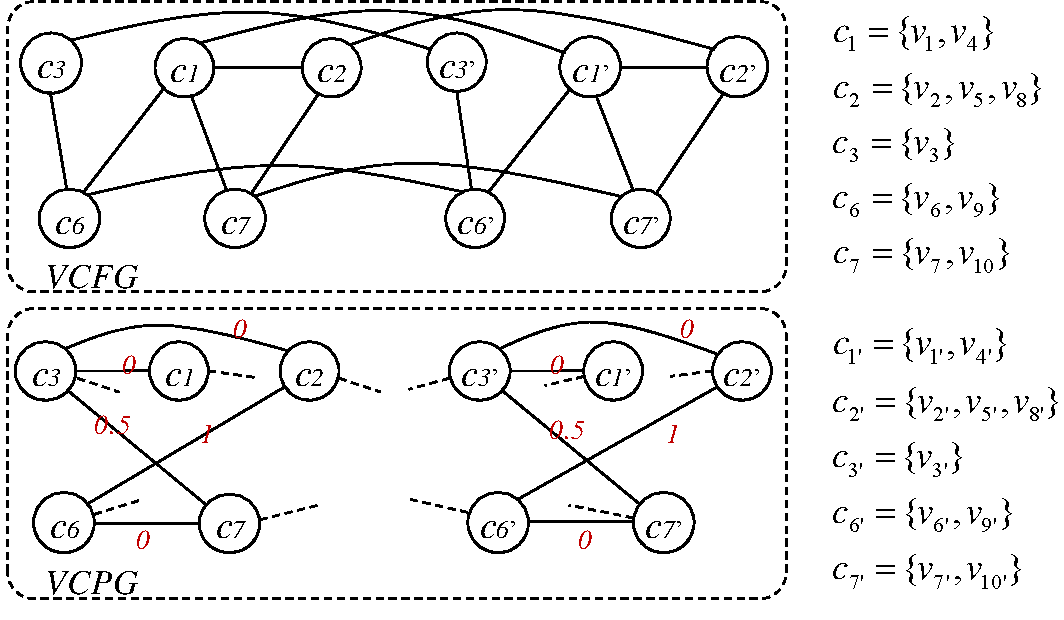
\includegraphics[width=8.6cm]{figure/vcg_c_1.pdf}\label{subfig:vcg_c_1}
}\\\hspace*{-1.2em}
\subfigure [] {
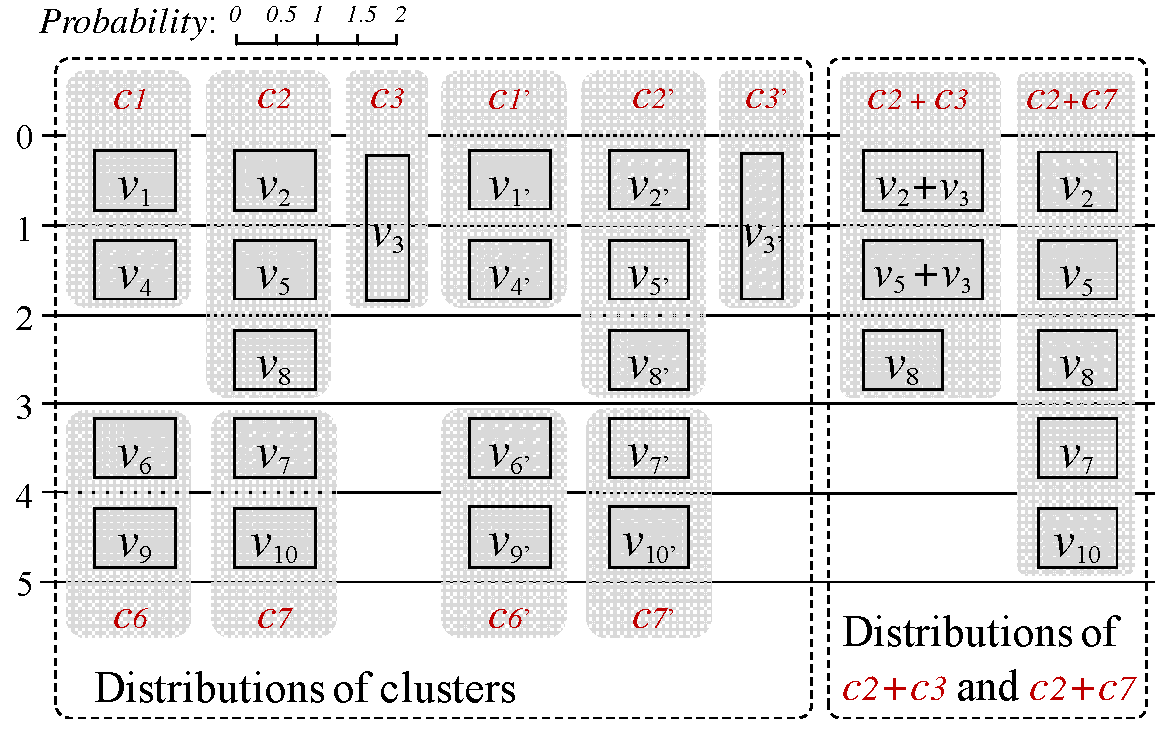
\includegraphics[width=8.8cm]{figure/vcg_c_2.pdf}\label{subfig:vcg_c_2}
}
\end{tabular}
\caption{Example of evaluating vendor compatible graph. \subref{subfig:vcg_c_1} $VCFG$ and $VCPG$ derived from task clustering results. \subref{subfig:vcg_c_2} Distributions of clusters.}
\label{fig:vc_c}
\end{figure}





\begin{figure*}[!t]
\centering
\begin{tabular}{ccc}
\subfigure [] {
\hspace*{-1em}
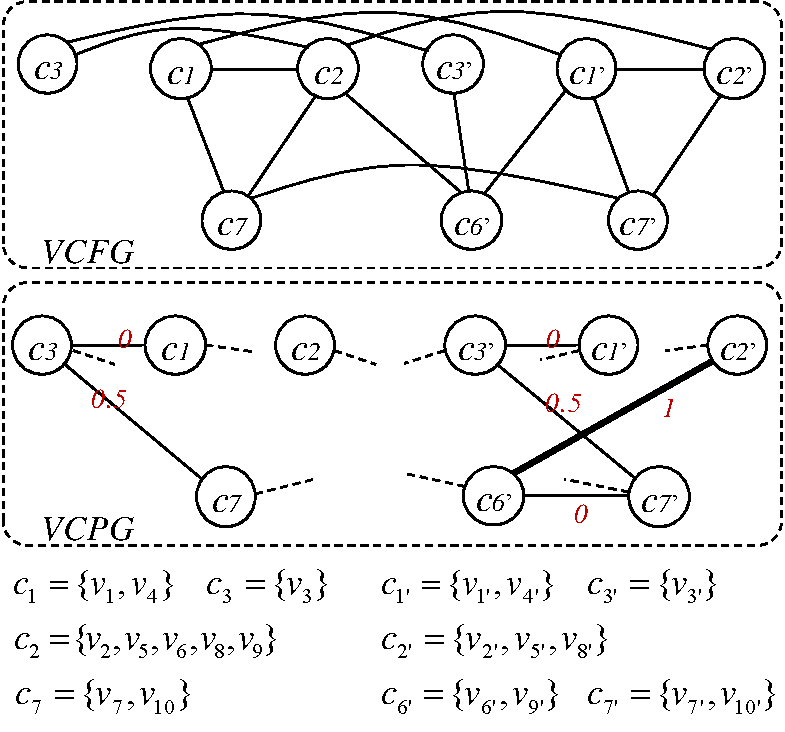
\includegraphics[width=5.8cm]{figure/vcg1.pdf}\label{subfig:assign1}
} &\hspace*{-1.5em}
\subfigure [] {
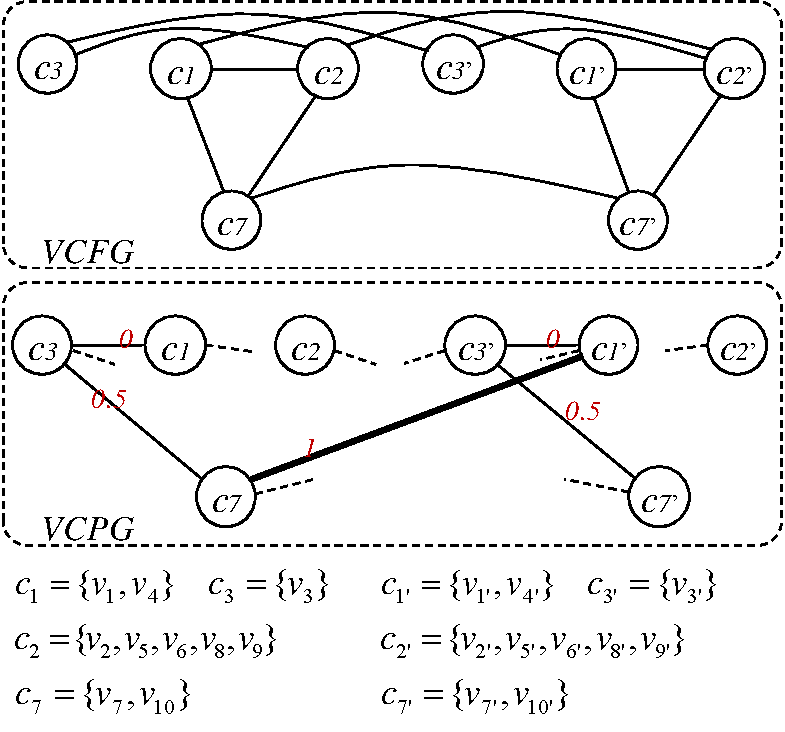
\includegraphics[width=5.8cm]{figure/vcg2.pdf}\label{subfig:assign2}
} &\hspace*{-1.5em}
\subfigure [] {
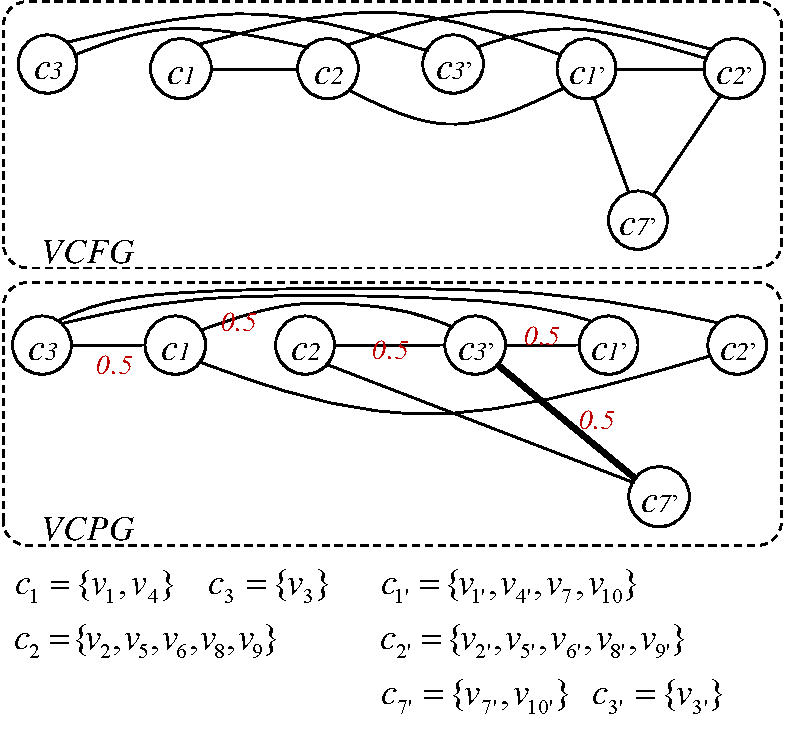
\includegraphics[width=5.8cm]{figure/vcg3.pdf}\label{subfig:assign3}
} \\\hspace*{-1em}
\subfigure [] {
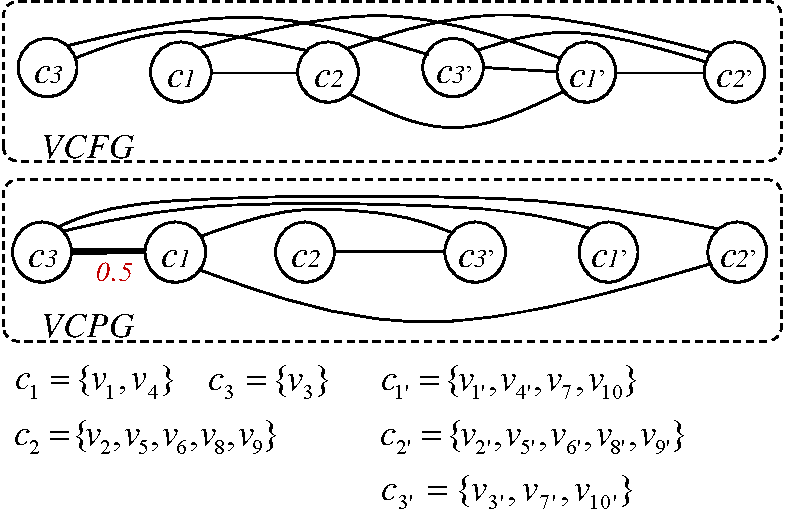
\includegraphics[width=5.8cm]{figure/vcg4.pdf}\label{subfig:assign4}
} &\hspace*{-1.5em}
\subfigure [] {
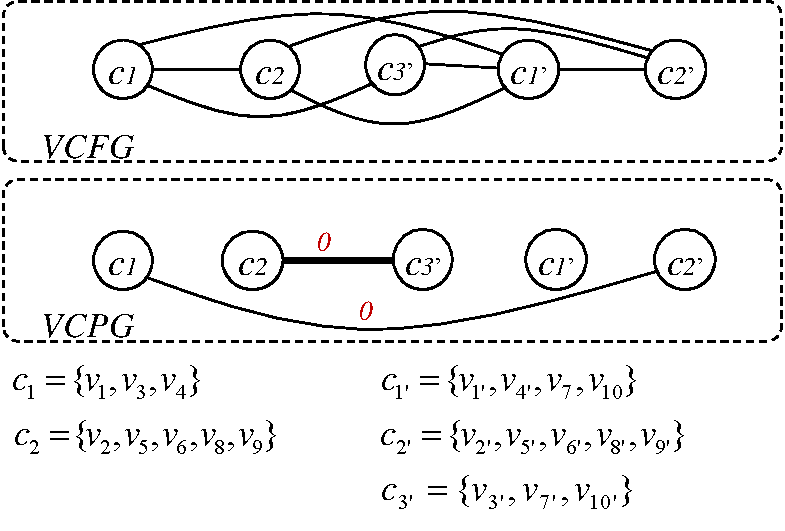
\includegraphics[width=5.8cm]{figure/vcg5.pdf}\label{subfig:assign5}
} &\hspace*{-1.5em}
\subfigure [] {
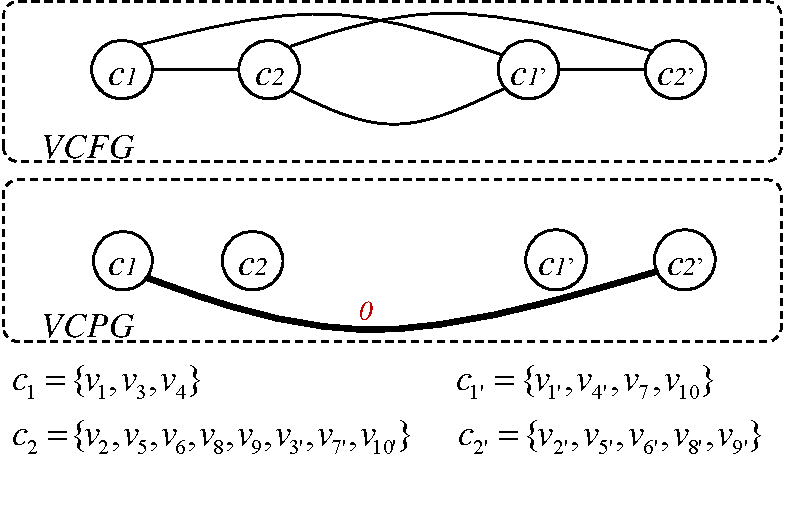
\includegraphics[width=5.8cm]{figure/vcg6.pdf}\label{subfig:assign6}
}
\end{tabular}
\caption{Example of cluster merging procedure. \subref{subfig:assign1} $VCFG$ and $VCPG$ in 2nd iteration of cluster merging. \subref{subfig:assign2} $VCFG$ and $VCPG$ in 3th iteration of cluster merging. \subref{subfig:assign3} $VCFG$ and $VCPG$ in 4th iteration of cluster merging. \subref{subfig:assign4} $VCFG$ and $VCPG$ in 5th iteration of cluster merging. \subref{subfig:assign5} $VCFG$ and $VCPG$ in 6th iteration of cluster merging. \subref{subfig:assign6} $VCFG$ and $VCPG$ in 7th iteration of cluster merging.}
\vspace*{-0.9em}
\label{fig:assign}
\end{figure*}



The number of cores required may be reduced by merging two clusters $c_i$ and $c_j$, which is denoted as $Merge(c_i, c_j)$, and it can be calculated as follows:
\begin{equation}
Merge(c_i, c_j) = DG_{max}(c_i) + DG_{max}(c_j) - DG_{max}(c_i+c_j)
\label{equ:weight_e2}
\end{equation}

A larger $Merge(c_i, c_j)$ indicates a higher probability that tasks in $c_i$ and $c_j$ can share the same cores, and therefore, assigning these tasks to the same IP vendor reduces the number of cores. Examples of calculating $Merge(c_2, c_3)$ and $Merge(c_2, c_7)$ are shown in Fig. \ref{subfig:vcg_c_2}. $Merge(c_2, c_3)=1+0.5-1.5=0$, which means that core reduction cannot be achieved by merging $c_2$ and $c_3$. $Merge(c_2, c_7)=1+1-1=1$, indicating that merging $c_2$ and $c_7$ may reduce one IP core.





$Merge(c_i, c_j)$ is then set as the weight of edge $(c_i, c_j)$ in $VCPG$. The edge with maximum weight is chosen, and the connected clusters are merged into one; this procedure continues until the number of clusters equals the number of vendors available. Because $VCPG$ with $O(n)$ nodes has nearly $O(n^2)$ edges, the maximum weight independent set of $VCPG$ is not introduced to determine the clusters to be merged due to its large time complexity.



An example of the cluster merging procedure is presented in Fig. \ref{fig:assign}, where the initial $VCFG$ and $VCPG$ are shown in Fig. \ref{subfig:vcg_c_1}, and the vendor constraint is 3. The maximum weight of all edges in $VCPG$ is 1, and $c_2$ and $c_6$ in Fig. \ref{subfig:vcg_c_1} are merged into one cluster, named $c_2$. All edges that once connected to $c_2$ and $c_6$ in $VCFG$ now connect to $c_2$ in the updated $VCFG$, and the weights of edges that connect to $c_2$ in $VCPG$ are also updated. Fig. \ref{subfig:assign1} shows $VCFG$ and $VCPG$ after the 1st iteration of merging clusters. Then, $c_2'$ and $c_6'$ are merged in the 2nd iteration because the weight of their connecting edge is 1. Fig. \ref{subfig:assign2} shows the updated $VCFG$ and $VCPG$. With the corresponding $VCFGs$ and $VCPGs$ shown in Fig. \ref{subfig:assign2}-Fig. \ref{subfig:assign6}, the pairs of clusters ($c_1'$, $c_7$), ($c_3'$, $c_7'$), ($c_1$, $c_3$), ($c_2$, $c_3'$) and ($c_1$, $c_2'$) are iteratively merged. This procedure terminates when the number of clusters equals the vendor constraint, and Fig. \ref{fig:assign_result} gives the final results, where the total estimated number of cores is 5.5.



Then, the number of timing-critical tasks in each cluster is countered, and the clusters containing more timing-critical tasks are assigned to the vendor with faster core speeds. Some timing-critical paths may be over-optimized because all tasks are treated with the lowest core speed in the performance-constrained task clustering stage, and we need to adjust the vendor assignment to meet more security constraints. The slacks of tasks are updated with the assigned core speeds, and every intra-core communication is checked in descending order of vulnerabilities $vul(e)$ to determine whether this communication can be reassigned with security constraints. An intra-core communication ($e$) can be reassigned to inter-core communication to satisfy security constraints only when all tasks in the paths that pass through $e$ have slack times no smaller than $dly(e)$, and one of its connected tasks will be assigned to the IP vendor with the least core increment.% This procedure is named as vendor assignment adjustment in the following discussion.


\begin{figure}[!t]
\centering
\hspace*{-0.8em}
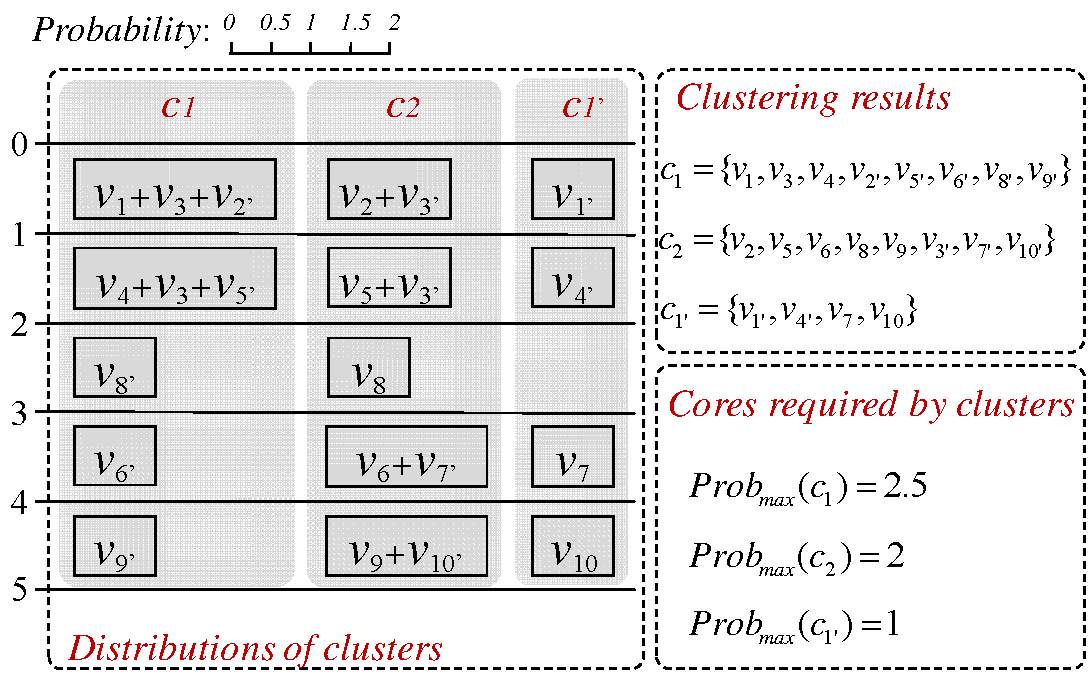
\includegraphics[width=8.8cm]{figure/vcg_result.pdf}
\caption{Cluster merging results under vendor constraint.}
\label{fig:assign_result}
\end{figure}

\begin{algorithm}[!b]
\caption{Vendor-assignment with core minimization, $vendor\_assign(TC, TC', vc, pc)$.}
\label{alg:VA}
{\textbf{Input:}}
performance-constrained clustering results of task\\
\hspace*{2.4em}  graph and duplicated task graph, $TC$, $TC'$.\\
\hspace*{2.4em} performance and vendor constraints, $pc$, $vc$.\\
%\hspace*{2.4em}  core speeds of vendors.\\
{\textbf{Output:}} vendor assignment, $VA$.
\begin{algorithmic}[1]
%\STATE calculate the mobility of of each task.
\STATE Calculate $DG_{max}(c)$ for each cluster $c$.
\STATE Construct $VCFG$ and weighted $VCPG$;
%\STATE Calculate the weights of edges in $VCPG$
\WHILE{$VCPG.node\_num > vc$}
\STATE Choose the edge $e_{max}=(c_i,c_j)$ with the maximum weight in $VCPG$, and merge $c_i$ and $c_j$ into one cluster.%, denoted as $c_{i}$.
\STATE Update $VCFG$ and weighted $VCPG$,
%\STATE Update the weights of edges that connect $c_i$ in $VCPG$.;
\ENDWHILE
%\STATE Count the number of timing critical tasks in each cluster;
\WHILE {Not all clusters are assigned with IP vendors}
    \STATE assign $c_i$ to vendor $vendor_j$, where $c_i$ is an unassigned cluster with the most timing critical tasks and $vendor_j$ is the available vendor with the fastest core speed.
\ENDWHILE
\STATE Update the distribution graphs with the determined task execution times and communication delays;
%\STATE Sort security constraint-violated edges in descending order of security loss;
\STATE $E_{cv}$ is the set consists of all intra-core communications;
\WHILE {$E_{cv}\neq \emptyset$}
\STATE Find $e\in E_{cv}$ with the largest $vul(e)$;
\IF{Assigning $e$ with security constraints still meets $pc$}
\STATE Assign either $source(e)$ or $target(e)$ with another vendor;
\STATE Update the distribution graphs;
\ENDIF
\STATE Remove $e$ from $E_{cv}$;
\ENDWHILE
\end{algorithmic}
\end{algorithm}




Algorithm \ref{alg:VA} describes the proposed vendor assignment algorithm. First (\textit{Lines 1-2}), the number of cores required by each cluster is estimated by $DG_{max}(c)$, and $VCFG$ and weighted $VCPG$ are constructed. Second (\textit{Lines 3-6}), the maximum weight edge in $VCPG$ is chosen, and the connected clusters are merged into one cluster. Both $VCFG$ and weighted $VCPG$ are then updated, and this procedure continues until the number of clusters equals the number of IP vendors available. Third (\textit{Lines 7-10}), the cluster containing more timing-critical tasks is assigned to the IP vendor with faster core speed. Finally (\textit{Lines 11-19}), the unprotected edges are checked in descending order of vulnerabilities, and the vendor assignments are adjusted under performance constraints to further reduce the design's vulnerability.




\subsection{Procedure of the Proposed Task Scheduling Method}

With all security constraints satisfied, the number of IP vendors is always equal to the number of nodes in the maximum clique (denoted as \textit{maximum clique size}) of $VCFG$. However, performance-constrained task clustering and vendor assignment may potentially increase the number of vendors required, and we must check every contracted edge if the resulting maximum clique size exceeds the vendor constraint. Computing the maximum clique size of a graph is NP-complete, and an efficient heuristic approach \cite{article:CL} is introduced. Each time after determining a contracted edge, the impact on the maximum clique size of the corresponding $VCFG$ is evaluated, and the edge is not contracted if the vendor constraint is violated. Instead, the algorithm chooses the second-best solutions.




\begin{algorithm}[!h]
\caption{Security-aware task scheduling with performance constraints, $task\_schedule(TG, pc, vc)$.}
\label{alg:PCTS}
{\textbf{Input:}} task graph, $TG$\\
\hspace*{2.4em} performance and vendor constraints, $pc$, $vc$.\\
%\hspace*{2.4em}  core speeds of vendors.\\
{\textbf{Output:}} scheduling results, $TS$.
\begin{algorithmic}[1]
\STATE $TC=task\_cluster(TG,pc)$;
\STATE $TC'=task\_cluster(TG',pc)$, where $TG'$ is the duplicate of $TG$;
\STATE $VA=vendor\_assign(TC, TC', vc, pc)$;
%\STATE $VA=vendor\_adjust(VA)$;
\FOR{each vendor $vendor_i$}
    \STATE $V_{vendor_i}$ is the set of all tasks assigned to $vendor_i$;
%    \STATE Calculate the mobilities of tasks in $V_{vendor_i}$;
    \STATE $FDS(V_{vendor_i}, pc)$;% using Force-directed scheduling;
\ENDFOR
\end{algorithmic}
\end{algorithm}


After vendor assignment, tasks with the same IP vendor are scheduled together using the force-directed scheduling (FDS) method \cite{article:PP}. FDS schedules tasks evenly across each time period, requiring only a small number of cores. Algorithm \ref{alg:PCTS} gives the whole procedure of the proposed task scheduling algorithm. Tasks in the task graph and duplicated task graph are clustered under the performance constraint $p_c$ (\textit{Lines 1-2}) and then assigned to IP vendors with a minimized number of cores required (\textit{Line 3}). Finally, tasks in each IP vendor are scheduled concurrently by the FDS (\textit{Lines 4-7}).% In this study, two types of security constraints are considered, and when more types of security constraints are introduced, our proposed method can be easily adopted and applied.

Our proposed methods can also be easily adopted in other actual scenarios. In the first scenario, the number of vendors available might be less than the maximum clique size of the corresponding $VCFG$. In this situation, a vendor-constrained task clustering method \cite{article:NW} can be introduced before vendor assignment, so that the vendor constraint can be satisfied with a minimized number of contracted edges. In the second scenario, application-specific IPs might not be able to support every task. For each type of IP, we first build its $VCFG$ and $VCPG$ according to the clustering results of tasks that belong to this type, and then perform the vendor assignment along with task scheduling individually.

\subsection{Time Complexity Analysis}

The time complexity of the proposed method is analyzed as follows, and the input task graph has $n$ nodes and $m$ edges.

In each iteration of the performance-constrained task clustering stage, constructing $ECCG$ from $TVG$ requires $O(m^2)$, and finding the MWIS in $ECCG$ also requires $O(m^2)$ \cite{conference:LC}. Only a constant number of iterations are conducted before reaching the performance constraint, and finding all contracted edges to meet the performance constraint requires $O(m^2)$. In addition, each time before contracting an edge, updating $VCFG$ and evaluating its impact on the maximum clique size requires $O(n^2)$, and only a limited number of edges are contracted, making its computational cost remains at $O(n^2)$. The total time complexity of performance-constrained task clustering is $O(m^2)$ (because $O(n)\leq O(m)$).

In the vendor assignment and task scheduling stage, constructing $VCFG$ and $VCPG$ requires $O(n^2)$. In each iteration of merging clusters, $O(m)$ is required to estimate the maximum clique size, and $O(n)$ is required to update both $VCFG$ and $VCPG$. Vender assignment requires $O(n)$ iterations of merging clusters, and its time complexity is $O(mn)$. Performing the force-directed scheduling method to schedule all tasks requires $O(n^2)$, and the total time complexity of the vendor assignment and task scheduling stage is $O(mn)$.

The sum of $O(m^2)$ and $O(mn)$ is $O(m^2)$, which is the total time complexity of the proposed method.


\section{Experimental Results}

\subsection{Experimental Setups}
All experiments were implemented in C on a Linux Workstation with an E5 2.6-GHz CPU and 32-GB RAM. We tested eight benchmarks from two sources\footnote{https://www.kasahara.cs.waseda.ac.jp/schedule/index.html.}: task graphs modeled from real application programs, including robot control (robot), sparse matrix solver (sparse), and SPEC fpppp (fpppp); and randomly generated task graphs (rnc500, rnc1000, rnc2000, rnc3000 and rnc5000). To simplify the experiments, all intra-core communication delays were ignored, and we set the step of core speed differences equal to 5\% of the fastest core speed.

\begin{table}[!h]
\renewcommand{\arraystretch}{1.1}
\caption{Details of Benchmarks}
\centering
\begin{tabular}{c|c|c|c|c|c}
\hline
\hline

task    &\multicolumn{1}{c|}{\multirow{2}{*}{$n$}}     &\multicolumn{1}{c|}{\multirow{2}{*}{$m$}}     &\multicolumn{1}{c|}{\multirow{2}{*}{Para. }}  &ACC   &\multicolumn{1}{c}{\multirow{2}{*}{\textit{maxClique}}}  \\
graph   &                                            &           &        & ($ut$)          &       \\
\hline
\hline

robot   &88   &131     &4.4 &28.2   &3 \\

sparse  &96   &67    &16.0  &20.2   &3 \\

fpppp   &334   &1145    &6.7  &21.3    &3  \\

rnc500  &500   &1910    &27.7  &10.6    &3  \\

rnc1000  &1000   &3005   &60.2  &7.8  &3 \\

rnc2000   &2000   &3930   &151.9  &10.6  &3 \\

rnc3000   &3000   &39034    &34.2 &13.0   &4  \\

rnc5000   &5000   &55432   &90.8  &11.0  &4 \\

\hline
\hline
\end{tabular}
\label{table:detail}
\end{table}


\begin{table*}[!t]
\renewcommand{\arraystretch}{1.1}
\caption{Performance-Constrained Task Scheduling Results on Real Application Graphs.}
\centering
\begin{tabular}{c|c|c|c|cccc|cccc|cccc}
\hline
\hline
task                                      &\multicolumn{1}{c|}{\multirow{2}{*}{$CCR$}}     &SL       &$pc$      &\multicolumn{4}{c|}{$vul_s~(10^{-3})$}        &\multicolumn{4}{c|}{Num. of cores}    &\multicolumn{4}{c}{average runtime ($s$)}    \\ \cline{5-8} \cline{9-12} \cline{13-16}
graph                                                                               &                                                &($ut$)   &($ut$)    &C-B  &MC-B &PSO-B   &Our   &C-B      &MC-B  &PSO-B  &Our    &C-B       &MC-B  &PSO-B  &Our  \\

\hline
\hline

\multicolumn{1}{c|}{\multirow{2}{*}{robot}}       &0.5  &839   &671  &353.68    &206.57   &163.82  &155.35    &14    &12  &11  &11    &3.9     &17.5  &221.6  &18.7            \\
                                                  &1.0  &1114  &892  &274.91    &185.62   &158.19  &147.83    &14    &12  &10  &10    &3.9     &17.6  &227.5  &18.9             \\
\hline

\multicolumn{1}{c|}{\multirow{2}{*}{sparse}}     &0.5 &179 &143 &146.75   &93.48   &81.48  &76.07    &21    &18  &16  &16    &5.3     &41.2  &285.6  &33.8          \\
                                                  &1.0 &236  &189 &157.48   &98.47   &86.53  &83.59    &19    &18  &16  &15    &5.5     &42.3  &288.3  &34.5            \\

\hline

\multicolumn{1}{c|}{\multirow{2}{*}{fpppp}}        &0.5 &1590  &1272  &15.23    &6.37    &5.15  &4.52    &13    &12  &10  &10    &7.5     &50.2  &369.2  &47.6             \\
                                                    &1.0 &2119  &1695  &11.49    &6.85   &5.39  &4.97    &12    &11  &10  &10    &8.3     &53.5  &372.7  &49.8            \\

\hline
\multicolumn{1}{c|}{\multirow{2}{*}{avg.}}      &0.5 &      &  &171.89  &102.14   &83.48   &78.65  & & &  &   &  & &         \\
                                                &1.0 &     &  &147.96  &96.98   &83.37   &78.80  & &  & &  &  & &         \\

\hline
\hline
\end{tabular}
\label{table:PCTS_A}
\end{table*}
%To test the performance of our proposed methods, a set of benchmarks is tested, and




\begin{table*}[!t]
\renewcommand{\arraystretch}{1.1}
\caption{Performance-Constrained Task Scheduling Results on Randomly Generated Task Graphs.}
\centering
\begin{tabular}{c|c|c|c|cccc|cccc|cccc}
\hline
\hline
task                                     &\multicolumn{1}{c|}{\multirow{2}{*}{$CCR$}}     &SL       &$pc$      &\multicolumn{4}{c|}{$vul_s~(10^{-3})$}        &\multicolumn{4}{c|}{Num. of cores}    &\multicolumn{4}{c}{average runtime ($s$)}    \\ \cline{5-8} \cline{9-12} \cline{13-16}
graph                                    &                                                &($ut$)   &($ut$)    &C-B    &MC-B  &PSO-B   &Our   &C-B       &MC-B  &PSO-B  &Our    &C-B       &MC-B  &PSO-B  &Our  \\

\hline
\hline
\multicolumn{1}{c|}{\multirow{2}{*}{rnc500}}      &0.5 &280 &224  &25.13       &15.70  &13.25  &12.46    &68    &65  &58  &58    &18.9     &113.6  &823.5  &95.4               \\
                                                  &1.0  &373  &300   &20.41    &16.35  &13.48  &12.95    &67    &63  &58  &56    &20.3     &121.3  &827.1  &98.7               \\
\hline
\multicolumn{1}{c|}{\multirow{2}{*}{rnc1000}}     &0.5 &190 &152  &47.92    &33.94   &27.82  &26.71    &95    &88  &79  &78    &38.8     &259.3  &3271.3  &183.5             \\
                                                  &1.0 &254  &203  &48.73    &31.95  &25.78  &23.69    &87    &81  &76  &74    &42.1     &273.3 &3282.9   &189.7              \\

\hline
\multicolumn{1}{c|}{\multirow{2}{*}{rnc2000}}     &0.5 &199  &159  &20.61    &16.53  &12.76  &12.37    &217    &184  &170  &167    &57.5     &715.7  &8661.3  &553.6             \\
                                                  &1.0 &268  &214  &21.47    &14.51  &11.34  &10.62    &206    &180  &168  &164    &59.1     &748.2  &8678.2  &572.9            \\

\hline
\multicolumn{1}{c|}{\multirow{2}{*}{rnc3000}}     &0.5 &1336  &1069  &56.41    &43.27  &36.73  &35.58    &73    &67  &64  &62    &182.5     &3582.6  &33425.6  &3014.9             \\
                                                  &1.0 &1779  &1423  &53.49    &37.74  &32.05  &31.18    &68    &62  &56  &56    &192.2     &3715.3  &33581.4  &3253.4            \\
\hline

\multicolumn{1}{c|}{\multirow{2}{*}{rnc5000}}       &0.5 &850  &680  &48.13    &43.17  &35.21  &34.52    &142    &132  &125  &122    &384.9     &9004.5  &91423.9  &6764.2             \\
                                                    &1.0 &1146 &917  &54.84    &47.25  &36.89  &36.55    &137    &125  &118  &115    &395.4     &9528.3  &91658.5  &6816.1            \\

\hline
\multicolumn{1}{c|}{\multirow{2}{*}{avg.}}       &0.5 &      &  &39.64  &30.52  &25.15    &24.33   &  & &  &   & &  &         \\
                                                 &1.0 &     &  &39.79  &29.56   &23.91   &23.01  & &  &  & &   &    &     \\
\hline
\hline
\end{tabular}
\label{table:PCTS_R}
\end{table*}

Table \ref{table:detail} lists the details of these benchmarks. Columns $n$ and $m$ give the numbers of tasks and communications in each task graph, respectively. Column Para. shows the parallelism of each task graph, which is the ratio of the total processing time of all tasks to the ASAP schedule length (without communication delays). Column ACC shows the average computational cost of each task. Considering that the maximum clique sizes of most task graphs modeled from real application programs are no larger than 4\cite{article:CL}, the maximum clique sizes (see column \textit{maxClique}) of all randomly generated $TGs$ in Table \ref{table:detail} are 3 or 4, and the IP vendor constraint is set to be the maximum clique size of the benchmark.


\textbf{Our} proposed method is then compared with three other methods to demonstrate its effectiveness. The first approach is the ``\textit{cluster-based approach}'' (\textbf{C-B} for short) \cite{article:CL}. This approach optimizes the schedule length by placing critical tasks on a single core, and then colors the performance-driven schedule to fulfill security constraints. The second approach is the ``\textit{min-cut-based approach}'' (\textbf{MC-B} for short) \cite{article:NW}. This approach boosts performance by iteratively contracting the edges selected by the max-flow min-cut algorithm, then assigns tasks to the IP vendor with the traditional graph coloring method, and finally schedules tasks with the force-directed scheduling-based method. The third approach is the ``\textit{PSO-based approach}'' (\textbf{PSO-B} for short) \cite{article:SR}, which uses a PSO-based method to find a resource-optimized solution with all security constraints satisfied. In the experiment, the accumulated vulnerabilities of unprotected communications are also added to the cost function of PSO-B, so that PSO-B can be used to find solutions with tight performance constraints.

%The \textbf{PSO-B} method \cite{article:SR} uses a PSO-based method to find a solution with minimized resource requirements. The \textbf{C-B} method \cite{article:CL} optimizes the schedule length by placing critical tasks on a single core, and conducts IP vendor assignment using the traditional graph coloring method. The \textbf{MC-B} method \cite{article:NW} boosts performance by iteratively contracting the edges selected by the max-flow min-cut algorithm and schedules tasks with the force-directed scheduling-based method.% and assigns tasks% with IP vendors while considering% the core speed variation.



\begin{figure*}[!t]
\centering
\begin{tabular}{ccc}
\subfigure [] {
\hspace*{-1.5em}
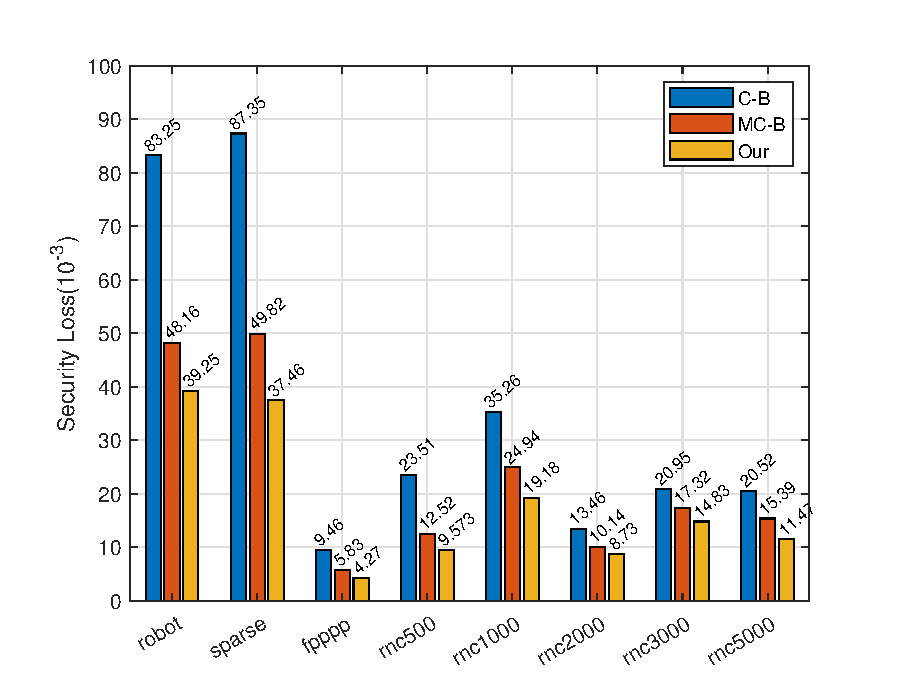
\includegraphics[width=6.4cm]{figure/randomly_set.eps}\label{subfig:rand_risk}
} &\hspace*{-2.8em}
\subfigure [] {
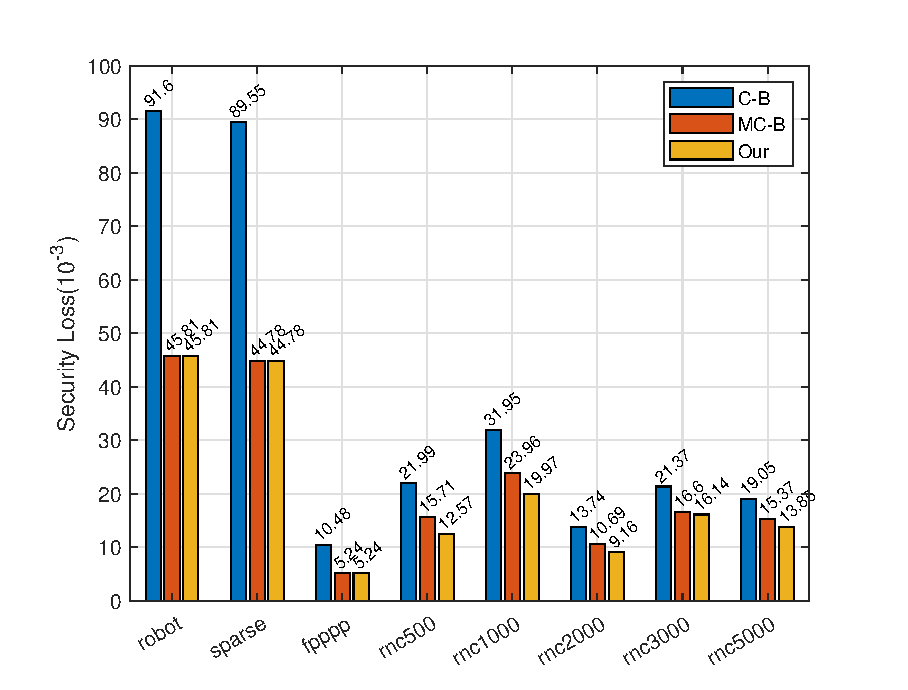
\includegraphics[width=6.4cm]{figure/equally_set.eps}\label{subfig:equ_risk}
} &\hspace*{-2.8em}
\subfigure [] {
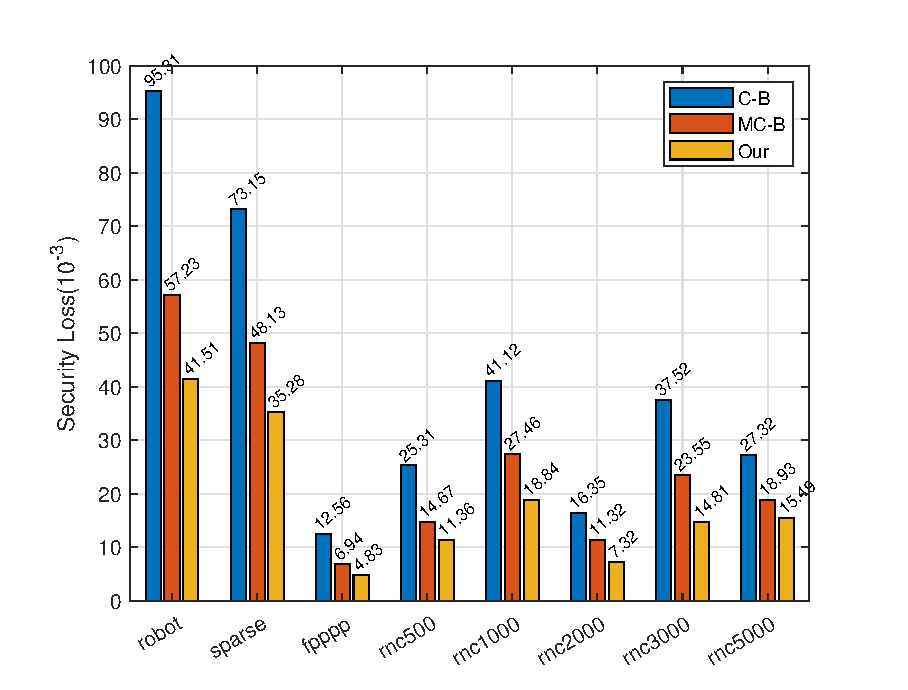
\includegraphics[width=6.4cm]{figure/linearly_set.eps}\label{subfig:linear_risk}
}
\end{tabular}
\caption{Comparison of design's vulnerabilities against hardware Trojan attacks. \subref{subfig:rand_risk} Design's vulnerability evaluations with vulnerabilities \textit{randomly set}. \subref{subfig:equ_risk} Design's vulnerability evaluations with vulnerabilities \textit{equally set}. \subref{subfig:linear_risk} Design's vulnerability evaluations with vulnerabilities \textit{linearly set}.}
\vspace*{-0.9em}
\label{fig:system_risk}
\end{figure*}


\subsection{Performance-Constrained Task Scheduling Results}

The performance-constrained task scheduling results are shown in Tables \ref{table:PCTS_A} and \ref{table:PCTS_R}. The communication-to-computation ratio ($CCR$) is the ratio of the inter-core communication delay to the computational cost of the task, and two $CCRs$ (0.5 and 1.0) are tested. The performance constraint is set to \textit{pc}=0.8\textit{SL}, where $SL$ is the ASAP schedule length with all security constraints satisfied. In this set of experiments, the communications have different vulnerabilities to hardware Trojan insertions, and to simplify our experiments, we set the vulnerability of $e_{ij}$ in $TG$ or $TG'$ as follows:

\begin{equation}
 vul(e_{ij})=\frac{2*dist(e_{ij})*pte}{SL*m}
\label{equ:risk_set1}
\end{equation}

\noindent where $dist(e_{ij})$ is the distance from $s$ to $v_i$. $pte$ is the \textit{possible Trojan entries} \cite{article:SR}, and we set $pte$ equal to 3 for all benchmarks.

Table \ref{table:PCTS_A} compares the task scheduling results of these methods on three real application graphs. The results show that our proposed method obtained the lowest $vul_s$ for all benchmarks. MC-B optimized the design's vulnerability by reducing the number of unprotected communications but ignored the vulnerability variation of communications. MC-B might also choose brother edges to contract, resulting in a $vul_s$ larger than that of our proposed method. PSO-B explores the design space to find the near-optimal solution, and the quality of its output also depends on the iteration of the algorithm. Furthermore, MC-B forgot to optimize the number of cores in the vendor assignment stage, and it required more cores than our method. Regarding the method C-B, it ignored both the design's vulnerability and the number of cores required during task scheduling, and both the $vul_s$ and number of cores are the largest among the compared methods. PSO-B outputs the schedules with low $vul_s$ and small numbers of cores required, but its CPU runtimes are much larger.

The comparison results of five randomly generated task graphs are shown in Table \ref{table:PCTS_R}. The number of edges in these task graphs is much larger than the edges of \textit{robot}, \textit{sparse}, and \textit{fpppp}, and therefore, the vulnerability of each communication is relatively much smaller (refer to Equ. (\ref{equ:risk_set1})). The comparison results show that our proposed method also obtained the best results in reducing both the $vul_s$ and the number of cores.

In terms of algorithm runtime, all of the algorithms can produce solutions within several minutes for the benchmarks modeled from real applications (see Table \ref{table:PCTS_A}). For benchmarks that contain many nodes and edges, such as \textit{rnc5000} which has 5000 nodes and 55432 edges (see Table \ref{table:PCTS_R}), our proposed method can output a solution within approximately 10 minutes, which indicates that our proposed method is applicable for most benchmarks in real practice.


\begin{table*}[t]
\renewcommand{\arraystretch}{1.1}
\caption{Comparisons of Cores Required.}
\centering
\begin{tabular}{c|c|ccccc|ccccccccc}
\hline
\hline
\multicolumn{1}{c|}{\multirow{2}{*}{task}}        &\multicolumn{1}{c|}{\multirow{2}{*}{\textit{SL}}}           & \multicolumn{5}{c|}{Loose vendor constraints}        & \multicolumn{8}{c}{Tight vendor constraints}         \\  \cline{3-7} \cline{8-16}

\multicolumn{1}{c|}{\multirow{2}{*}{graph}}       &\multicolumn{1}{c|}{\multirow{2}{*}{($ut$)}}     &\multicolumn{1}{c}{\multirow{2}{*}{$vc$}}   & \multicolumn{4}{|c|}{Num. of cores}  &\multicolumn{1}{c}{\multirow{2}{*}{$vc$}}   & \multicolumn{4}{|c}{Num. of cores}    & \multicolumn{4}{|c}{Proportion of unprotected edges}    \\ \cline{4-7} \cline{9-12}  \cline{13-16}

                           &    &    & \multicolumn{1}{|c}{\multirow{1}{*}{C-B}}         &MC-B  &PSO-B   &~~Our~~  &     &\multicolumn{1}{|c}{\multirow{1}{*}{C-B }}        &MC-B    &PSO-B &~~Our~~    &\multicolumn{1}{|c}{\multirow{1}{*}{C-B}}        &MC-B  &PSO-B   &~~Our~~     \\
\hline
\hline

robot              &1114  &3 &10 &9 &8 &8        &2     &10     &8  &7   &7       &2.29\%     &1.53\%   &1.53\%  &1.53\%  \\

sparse              &236  &3  &14 &12 &12 &12     &2     &14     &11  &10   &10     &8.96\%     &5.97\%   &5.97\%  &5.97\%  \\

fpppp              &2119  &3   &10 &9 &8 &8      &2     &9     &7   &6  &6      &1.57\%     &0.96\%   &0.96\%  &0.96\% \\

rnc500            &373    &3  &47 &45 &40 &39     &2     &42     &38   &36  &35      &4.50\%     &3.72\%  &3.72\%   &3.72\% \\

rnc1000            &254   &3   &68 &63 &58 &56    &2     &58     &51   &48  &47       &1.73\%     &1.30\%   &1.30\%  &1.30\%  \\

rnc2000           &268    &3  &156 &148 &132 &130     &2     &139     &127  &118   &116     &0.74\%     &0.46\%   &0.46\%  &0.46\% \\

rnc3000           &1779   &4   &56 &51 &48 &48       &2     &52     &48   &45  &45     &58.52\%     &53.15\%   &53.15\%  &53.15\% \\

rnc5000           &1146   &4   &106 &98 &90 &88      &2     &97     &91   &84  &83     &70.24\%     &67.89\%  &67.89\%   &67.89\%  \\

\hline
\hline
\end{tabular}
\label{table:core_usage}
\end{table*}


\subsection{Design's Vulnerability Optimization Results}

Then, the effectiveness of our method in optimizing the design's vulnerability is tested. $CCR$ is set to \textit{CCR}=1.0 for all benchmarks, and the performance constraint is set to $pc=0.9*SL$. Fig. \ref{fig:system_risk} shows the comparative results of design's vulnerabilities among C-B, MC-B, and our methods, with the following three sets of vulnerability configurations:


\begin{enumerate}
\item \textbf{Randomly Set}: the vulnerabilities of communications are randomly set with the value among [0, $\frac{2*pte}{m}$];
\item \textbf{Equally Set}: the vulnerabilities of all communications are the same, with the value of $\frac{pte}{m}$;
\item \textbf{Linearly Set}: the communication closer to the source has higher vulnerability, and the vulnerability of $e_{ij}$ is set as $vul(e_{ij})=\frac{2*(SL-dist(e_{ij}))*pte}{SL*m}$;
\end{enumerate}



The $pte$ is set to 3 in this set of experiments. Because both C-B and MC-B ignore the vulnerability variation, they produced the same task scheduling result with different vulnerability configurations. Our proposed method seeks the task schedule with the lowest design's vulnerability, and produces different task scheduling results for different vulnerability configurations.


Figs. \ref{subfig:rand_risk}, \ref{subfig:equ_risk}, and \ref{subfig:linear_risk} show the design's vulnerability with the vulnerabilities of communications \textit{randomly set}, \textit{equally set}, and \textit{linearly set}, respectively. For each tested benchmark, our proposed method outperforms both C-B and MC-B with different vulnerability configurations, and detailed comparisons are given as follows:


\begin{enumerate}
    \item When the vulnerabilities are \textit{randomly set}, the averaged design's vulnerabilities of C-B and MC-B are 36.72*$10^{-3}$, and 23.02*$10^{-3}$, respectively, and our proposed method obtains the lowest design's vulnerability, which is only 18.11*$10^{-3}$.
    \item If the vulnerabilities are \textit{equally set}, our method and MC-B obtain nearly equivalent results because MC-B treats each communication equally when optimizing system performance. The averaged design's vulnerabilities of C-B, MC-B and our methods are 37.47*$10^{-3}$, 22.27*$10^{-3}$, and 20.94*$10^{-3}$, respectively.
    \item If the vulnerabilities are \textit{linearly set}, our proposed method still demonstrate its advantage by obtaining the lowest design's vulnerability, which is 18.68*$10^{-3}$. However, the averaged design's vulnerabilities of C-B and MC-B are 41.08*$10^{-3}$ and 26.03*$10^{-3}$, respectively.
    \item For some benchmarks (\textit{robot} and \textit{sparse}), their design's vulnerabilities are relatively high because the vulnerabilities of communications are also determined by the number of edges in task graphs. These task graphs have much fewer edges, making the values of vulnerabilities in \textit{robot} and \textit{sparse} much larger than that in the other task graphs.
\end{enumerate}





\subsection{Comparison of Cores Required}

To demonstrate the effectiveness of our method in reducing the number of cores required, the performance constraint is set to \textit{SL} so that the performance-constrained task clustering stage can be skipped. Table \ref{table:core_usage} shows the numbers of cores required, where two sets of vendor constraints are tested. The loose vendor constraints are first set for all benchmarks, and the vendor constraint is set to be the maximum clique size of the corresponding $TG$. C-B ignores core optimization, MC-B only minimizes the number of cores when scheduling tasks, and PSO-B explores the design space with a limited number of iterations. In our proposed method, reducing the number of cores is considered in both vendor assignment and task scheduling, which enlarges the optimization space for saving cores. The results indicate that our proposed method needs the fewest numbers of cores in all benchmarks, and MC-B, PSO-B and our proposed method reduce the numbers of cores by 8.44\%, 16.08\% and 17.11\%, respectively, compared to the C-B method.


Then, the tight vendor constraints are set because there might not be sufficient vendors for some specific IPs, and the vendor constraints of all benchmarks are set to 2. To meet the tight vendor constraints, the vendor-constrained task clustering method proposed in \cite{article:NW} is used to remove some security constraints from communications and allow the adjacent tasks to be executed on the cores from the same IP vendor. Therefore, some communications become unprotected, and the proportions of the number of unprotected edges to the number of all edges are given in the last column of Table \ref{table:core_usage}. Because MC-B, PSO-B and our method use the same vendor-constrained task clustering, the proportions of their unprotected edges are the same. C-B ignored reducing the number of unprotected edges to meet vendor constraints, and its numbers of unprotected edges are larger. For the benchmarks \textit{rnc3000} and \textit{rnc5000}, whose task graphs contain many 4-cliques, many edges become unprotected to satisfy the vendor constraint. The number of cores required shows that our proposed method also obtained the fewest cores among these four methods, and the average numbers of cores required by MC-B, PSO-B and our proposed method are 13.47\%, 20.68\% and 21.49\% less than that of C-B, respectively.





\section{Conclusions}

In this study, a security-driven task scheduling method is proposed to reduce the performance and area overheads of implementing security constraints in the design process, and the desired performance is set as a constraint. The communications between data-dependent tasks are treated with different vulnerabilities against hardware Trojan attacks, and a maximum weight independent set-based task clustering method is proposed to reduce the schedule length while maintaining a high security level. In addition, the numbers of cores required are optimized in both vendor assignment and task scheduling stages by assigning tasks that can share most cores to the same vendor and scheduling them evenly in each time period, which enlarges the optimization space for reducing cores. Experimental results demonstrate that our proposed method obtains the highest system security and the fewest cores among all compared methods.

%\bibliographystyle{ieicetr}% bib style
%\bibliography{}% your bib database
\begin{thebibliography}{99}% more than 9 --> 99 / less than 10 --> 9

\bibitem{article:KX}
K. Xiao, D. Forte, Y. Jin, R. Karri, S. Bhunia, and M. Tehranipoor, ``Hardware Trojans: lessons learned after one decade of research,'' \textit{ACM Transactions on Design Automation of Electronic Systems}, vol. 22, no. 1, pp. 6-29, May 2016.


\bibitem{conference:XW}
X. Wang and R. Karri, ``NumChecker: detecting kernel control-flow modifying rootkits by using hardware performance counters,'' \textit{Proc. Design Automation Conference}, pp. 1-7, May 2013.

%\bibitem{conference:XTN}
%X.T. Ngo, J.-L. Danger, S. Guilley, Z. Najm, and O. Emery, ``Hardware property checker for run-time hardware Trojan detection,'' \textit{Proc. European Conference on Circuit Theory and Design}, pp. 1-4, 2015.

\bibitem{article:SB}
S. Bhunia, M.S. Hsiao, M. Banga, and S. Narasimhan, ``Hardware Trojan attacks: threat analysis and countermeasures,'' \textit{Proceedings of the IEEE}, vol. 102, no. 8, pp. 1229-1247, Aug. 2014.

\bibitem{conference:MH}
M. Hussain, A. Malekpour, H. Guo, and S. Parameswaran, ``EETD: an energy efficient design for runtime hardware Trojan detection in untrusted network-on-chip,'' \textit{Proc. IEEE Computer Society Annual Symposium on VLSI}, pp. 345-350, 2018.


\bibitem{conference:AM1}
A. Malekpour, R. Ragel, A. Ignjatovic, and S. Parameswaran, ``DosGuard: protecting pipelined MPSoCs against hardware Trojan based DoS attacks,'' \textit{Proc. International Conference on Applications-specific Systems, Architectures and Processors}, pp. 45-52, 2017

\bibitem{conference:FK}
F. Kounelis, N. Sklavos, and P. Kitsos, ``Run-time effect by inserting hardware Trojans in combinational circuits,'' \textit{Euromicro Conference on Digital System Design}, pp. 287-290, 2017.




\bibitem{network:SS}
S. Swapp, \emph{Scanning Electron Microscopy (SEM)},\hskip 1em University of Wyoming.

%\bibitem{conference:MM}
%M. Banga and M.S. Hsiao, ``A novel sustained vector technique for the detection of hardware Trojans,'' \textit{Proc. International Conference of VLSI Design}, pp. 327-332, 2009.

\bibitem{conference:BB}
B. Bilgic and S. Ozev, ``Guaranteed activation of capacitive Trojan triggers during post production test via supply pulsing,'' \textit{Proc. Design, Automation \& Test in Europe Conference}, pp. 993-998, 2022.

%\bibitem{conference:KX}
%K. Xiao and M. Tehranipoor, ``BISA: Built-in self-authentication for preventing hardware Trojan insertion,'' \textit{Proc. International Symposium on Hardware-Oriented Security and Trust}, pp. 45-50, 2013.

\bibitem{article:DD}
D. Deng, Y. Wang, and Y. Guo, ``Novel design strategy toward A2 Trojan detection based on built-in acceleration structure,'' \textit{IEEE Transactions on Computer-Aided Design of Integrated Circuits and Systems}, vol. 39, no. 12, pp. 4496-4509, Feb. 2020.

\bibitem{article:YH1}
Y. Huang, S. Bhunia, and P. Mishra, ``Scalable test generation for Trojan detection using side channel analysis,'' \textit{IEEE Transactions on Information Forensics and Security}, vol. 13, no. 11, pp. 2746-2760, Nov. 2018.

%\bibitem{article:LN}
%L. Nguyen, C. Cheng, M. Prvulovic, and A. Zaji\'{c}, ``Creating a backscattering side channel to enable detection of dormant hardware Trojans,'' \textit{IEEE Transactions on Very Large Scale Integration (VLSI) Systems}, vol. 27, no. 7, pp. 1561-1574, Apr. 2019.


%\bibitem{article:SY}
%S. Yang, T. Hoque, P. Chakraborty, and S. Bhunia, ``Golden-free hardware Trojan detection using self-referencing,'' \textit{IEEE Transactions on Very Large Scale Integration (VLSI) Systems}, vol. 30, no. 3, pp. 325-338, Mar. 2022.




\bibitem{conference:YH}
Y. Hou, H. He, K. Shamsi, Y. Jin, D. Wu, H. Wu, ``R2D2: runtime reassurance and detection of A2 Trojan,'' \textit{Proc. International Symposium on Hardware-Oriented Security and Trust}, pp. 195-200, 2018.

%\bibitem{article:SB}
%S. Bhunia, M. Abramovici, D. Agrawal, P. Bradly, M.S. Hsiao, J. Plusquellic, and M. Tehranipoor, \textit{IEEE Design \& Test}, vol. 30, no. 3, pp. 6-17, May 2013.


%\bibitem{conference:JH}
%J. He, X. Guo, H. Ma, Y. Liu, Y. Zhao, and Y. Jin, ``Runtime trust evaluation and hardware Trojan detection using on-chip EM sensors,'' \textit{Proc. Design Automation Conference}, pp. 1-6, Jun. 2020.

%\bibitem{article:YH}
%Y. Hou, H. He, K. Shamsi, Y. Jin, D. Wu and H. Wu, ``On-chip analog Trojan detection framework for microprocessor trustworthiness,'' \textit{IEEE Transactions on Computer-Aided Design of Integrated Circuits and Systems}, vol. 38, no. 10, pp. 1820-1830, Oct. 2019.

%\bibitem{conference:AK}
%A. Kulkarni, Y. Pino, and T. Mohsenin, ``SVM-based real-time hardware Trojan detection for many-core platform,'' \textit{Proc. International Symposium on Quality Electronic Design}, pp. 362-367, 2016.

%\bibitem{article:AK}
%A. Kulkarni, Y. Pino, M. French, and T. Mohsenin, ``Real-time anomaly detection framework for many-core router through machine learning techniques,'' \textit{ACM Journal of Emerging Technologies in Computing Systems}, vol. 13, no. 1, pp. 10-22, Jan. 2017.

%\bibitem{article:HZ}
%H. Zhao, L. Kwiat, K.A. Kwiat, C.A. Kamhoua, and L. Njilla, ``Applying chaos theory for runtime hardware Trojan monitoring and detection,'' \textit{IEEE Transactions on Dependable and Secure Computing}, vol. 17, no. 4, pp. 716-729, Jul. 2020.

%\bibitem{conference:AM}
%A. Malekpour, R. Ragel, D. Murphy, A. Ignjatovic, and S. Parameswaran, ``Hardware Trojan detection and recovery in MPSoCs via on-line application specific testing,'' \textit{ACM Journal of Emerging Technologies in Computing Systems}, vol. 13, no. 1, pp. 10-22, Jan. 2017.

%\bibitem{article:BM}
%B.J. Mohd, S. Abed, T. Hayajneh, and M.H. Alshayeji, ``Run-time monitoring and validation using reverse funciton (RMVRF) for hardware Trojans detection,'' \textit{IEEE Transactions on Dependable and Secure Computing}, vol. 18, no. 6, pp. 2689-2704, Nov. 2021.

%\bibitem{article:CB}
%C. Bao, D. Forte, and A. Srivastava, ``Temperature tracking: toward robust run-time detection of hardware Trojans,'' \textit{IEEE Transactions on Computer-Aided Design of Integrated Circuits and Systems}, vol. 34, no. 10, pp. 1577-1585, Oct. 2015.

%\bibitem{article:JZ}
%J. Zhu \textit{et al.}, ``Jintide: utilizing low-cost reconfigurable external monitors to substantially enhance hardware security of large-scale CPU clusters,'' \textit{IEEE Journal of Solid-State Circuits}, vol. 56, no. 8, pp. 2585-2601, Aug. 2021.

%\bibitem{article:FK}
%F. Khalid, S.R. Hasan, S. Zia, O. Hasan, F. Awwad, and M. Shafique, ``MacLeR: machine learning-based runtime hardware Trojan detection in resource-constrained IoT edge devices,'' \textit{IEEE Transactions on Computer-Aided Design of Integrated Circuits and Systems}, vol. 39, no. 11, pp. 3748-3761, Nov. 2020.




\bibitem{article:JR3}
J. Rajendran, O. Sinanoglu, and R. Karri, ``Building trustworthy systems using untrusted components: a high-level synthesis approach,'' \textit{IEEE Transactions on Very Large Scale Integration (VLSI) Systems}, vol. 24, no. 9, pp. 2946-2959, Apr. 2016.

%\bibitem{article:SS}
%S. Sethumadhavan, A. Waksman, M. Suozzo, Y. Huang, and J. Eum, ``Trustworthy hardware from untrusted components,'' \textit{Communications of the ACM}, vol. 58, no. 9, pp. 60-71, Sep. 2015.

\bibitem{article:TR}
T. Reece and W. H. Robinson, ``Detection of hardware Trojan in third-party intellectual property using untrusted modules,'' \textit{IEEE Transactions on Computer-Aided Design of Integrated Circuits and Systems}, vol. 35, no. 3, pp. 357-366, Jul. 2015.

\bibitem{conference:MB}
M. Beaumont, B. Hopkins, and T. Newby, ``SAFER PATH: security architecture using fragmented execution and replication for protection against Trojaned hardware,'' \textit{Proc. Design, Automation \& Test in Europe Conference}, pp. 1000-1005, Mar. 2012.

\bibitem{conference:XC}
X. Cui et al., ``High-level synthesis for run-time hardware Trojan detection and recovery,'' \textit{Proc. Design Automation Conference}, pp. 1-6, Jun. 2014.

\bibitem{conference:MS}
M. Shatta, I. adly, H. Amer, G. Alkady, R. Daoud, S. Hamed, and S. Hatem, ``FPGA-based architectures to recover from hardware Trojan horses, single event upsets and hard failures,'' \textit{Proc. International Conference on Microelectronics}, pp. 1-4, 2020.

\bibitem{conference:JR2}
J. Rajendren, H. Zhang, O. Sinanoglu, and R. Karri, ``High-level Synthesis for Security and Trust,'' \textit{Proc. International On-Line Testing Symposium}, pp. 232-233, 2013.

\bibitem{article:SR}
S. Rajmohan, N. Ramasubramanian, and N. Naganathan, ``Hybrid evolutionary design space exploration algorithm with defence against third party IP vulnerabilities,'' \textit{IEEE Transactions on Computer-Aided Design of Integrated Circuits and Systems}, vol. 39, no. 10, pp. 2602-2614, May 2022.

\bibitem{conference:AS}
A. Sengupta and S. Bhadauria, ``Untrusted third party digital IP cores: power-delay trade-off driven exploration of hardware Trojan secuired datapath during high level synthesis,'' \textit{Proc. Great Lakes Symposium on VLSI}, pp. 167-172, May 2015.

\bibitem{article:YS}
Y. Sun, G. Jiang, S.-K. Lam, and F. Ning, ``Designing energy-efficient MPSoC with untrustworthy 3PIP cores,'' \textit{IEEE Transactions on Parallel and Distributed Systems}, vol. 31, no. 1, pp. 51-63, Jan. 2020.

\bibitem{article:XC}
X. Cui, X. Zhang, H. Yan, L. Zhang, K. Cheng, Y. Wu, and K. Wu, ``Toward building and optimizing trustworthy systems using untrusted components: a graph-theoretic perspective,'' \textit{IEEE Transactions on Computer-Aided Design of Integrated Circuits and Systems}, vol. 41, no. 5, pp. 1386-1399, Oct. 2020.


\bibitem{article:CL}
C. Liu, J. Rajendran, C. Yang, and R. Karri, ``Shielding heterogeneous MPSoCs from untrustworthy 3PIPs through security-driven task scheduling,'' \textit{IEEE Transactions on Emerging Topics in Computing}, vol. 2, no. 4, pp. 461-472, Aug. 2014.

\bibitem{article:NW}
N. Wang, S. Chen, J. Ni, X. Ling, and Y. Zhu, ``Security-aware task scheduling using untrusted components in high-level synthesis,'' \textit{IEEE Access}, vol. 6, pp. 15663-15678, Jan. 2018.

\bibitem{conference:NW}
N. Wang, M. Yao, D. Jiang, S. Chen, and Y. Zhu, ``Security-driven task scheduling for multiprocessor system-on-chips with performance constraints,'' \textit{Proc. IEEE Computer Society Annual Symposium on VLSI}, pp. 545-550, 2018.


\bibitem{conference:HS}
H. Salmani and M. Tehranipoor, ``Analyzing circuit vulnerability to hardware Trojan insertion at the behavioral level,'' \textit{IEEE International Symposium on Defect and Fault Tolerance in VLSI and Nanotechnology Systems}, pp. 190-195, 2013.





\bibitem{article:WH}
W. Hu, C.-H. Chang, A. Sengupta, S. Bhunia, R. Kastner, H. Li, ``An overview of hardware security and trust: threats, countermeasures, and design tools,'' \textit{IEEE Transactions on Computer-Aided Design of Integrated Circuits and Systems}, vol. 40, no. 6, pp. 1010-1038, Jun. 2021.


%\bibitem{article:YC}
%Y. Cao, C.Q. Liu, and C.-H. Chang, ``A low power diode-clamped inverter-based strong physical unclonable function for robust and lightweight authentication,'' \textit{IEEE Transactions on Circuits and Systems I: Regular Papers}, vol. 65, no. 11, pp. 3864-3873, Nov. 2018.

%\bibitem{article:FP}
%F. Pareschi, G. Setti, and R. Rovatti, ``Implementation and testing of high-speed CMOS true random number generators based on chaotic systems,'' \textit{IEEE Transactions on Circuits and Systems I: Regular Papers}, vol. 57, no. 10, pp. 3124-3137, Dec. 2010.





%\bibitem{article:QS}
%Q. Shi, M.M. Tehranipoor, and D. Forte, ``Obfuscated built-in self-authentication with secure and efficient wire-lifting,'' \textit{IEEE Transactions on Computer-Aided Design of Integrated Circuits and Systems}, vol. 38, no. 11, pp. 1981-1994, Nov. 2019.

\bibitem{article:DM}
D. Meng, R. Hou, G. Shi, B. Tu, A. Yu, Z. Zhu, X. Jia, Y. Wen, and Y. Yang, ``Built-in security computer: deploying security-first architecture using active security processor,'' \textit{IEEE Transactions on Computers}, vol. 69, no. 11, pp. 1571-1583, Nov. 2020.

\bibitem{article:NH}
N. Hu, M. Ye, and S. Wei, ``Surviving information leakage hardware Trojan attacks using hardware isolation,'' \textit{IEEE Transactions on Emerging Topics in Computing}, vol. 7, no. 2, pp. 253-261, Apr. 2019.

%\bibitem{book:TA}
%T. Alves and D. Felton, ��TrustZone: Integrated hardware and soft ware security-enabling trusted computing in embedded systems,�� ARM, Cambridge, U.K., White Paper, 2014.


\bibitem{conference:HK}
H. Kim, S. Hong, B. Preneel, and I. Verbauwhede, ``STBC: Side channel attack tolerant balanced circuit with reduced propagation delay, \textit{Proc. IEEE Computer Society Annual Symposium on VLSI}, pp. 74-79, 2017.

%\bibitem{article:SP}
%S. Patranabis, A. Chakraborty, D. Mukhopadhyay, and P.P. Chakrabarti, ``Fault space transformation: a generic approach to counter differential fault analysis and differential fault intensity analysis on AES-like block ciphers,'' \textit{IEEE Transactions on Computer-Aided Design of Integrated Circuits and Systems}, vol. 12, no. 5, pp. 1092-1102, May 2017.

%\bibitem{article:AS0}
%A. Sengupta, D. Roy, and S.P. Mohanty, ``Triple-phase watermarking for reusable IP core protection during architecture synthesis,'' \textit{IEEE Transactions on Computer-Aided Design of Integrated Circuits and Systems}, vol. 37, no. 4, pp. 1092-1102, Apr. 2018.

\bibitem{article:AS1}
A. Sengupta and M.Rathor, ``IP core steganography for protecting DSP kernels used in CE systems,'' \textit{IEEE Transactions on Consumer Electronics}, vol. 65, no. 4, pp. 506-515, Nov. 2019.

\bibitem{article:SY1}
S. Yu, C. Gu, W. Liu, and M. O'Neill ``Deep learning-based hardware Trojan detection with block-based netlist information extraction,'' \textit{IEEE Transactions on Emerging Topics in Computing}, vol. 10, no. 4, pp. 1837-1853, Oct. 2022.

%\bibitem{article:WS}
%W. Shan, S. Zhang, J. Xu, M. Lu, L. Shi, and J. Yang, ``Machine learning assisted side-channel-attack countermeasure and its application on a 28-nm AES circuit,'' IEEE Journal of Solid-State Circuits, vol. 55, no. 33, pp. 794-804, Mar. 2020.


\bibitem{conference:XZ}
X. Zhang and M. Tehranipoor, ``Case study: detecting hardware Trojans in third-party deigital IP cores,'' \textit{International Symposium on Hardware-Oritented Security and Trust}, pp. 67-70, 2011.











\bibitem{article:MT}
M. Tehranipoor and F. Koushanfar, ``A survey of hardware Trojan taxonomy and detection,'' \textit{IEEE Design and Test of Computers}, vol. 27, no. 1, pp. 10-25, Jan. 2010.

\bibitem{article:JC}
J. Cruz, P. Slpsk, P. Gaikwad, and S. Bhunia, ``TVF: a metric for quantifying vulnerability against hardware Trojan attacks,'' \textit{IEEE Transactions on Very Large Scale Integration (VLSI) Systems}, vol. 31, no. 7, pp. 969-979, Jul. 2026.



\bibitem{article:YD}
Y. Dou, C. Gu, C. Wang, W. Liu, and F. Lombardi, ``Security and approximation: vulnerabilities in approximation-aware testing,'' \textit{IEEE Transactions on Emerging Topics in Computing}, vol. 11, no. 1, pp. 265-271, Jan. 2023.



\bibitem{article:SB1}
S. Bhunia, M. Abramovici, D. Agrawal, P. Bradley, M.S. Hsiao, J. Plusquellic, M. Tehranipoor, ``Protection against hardware Trojan attacks: towards a comprehensive solution,'' \textit{IEEE Design \& Test}, vol. 30, no. 3,  pp. 6-17, Jun. 2013.

%\bibitem{conference:RC}
%R.S. Chakraborty, S. Narasimhan, and S. Bhunia, ``Hardware Trojan: threats and emerging solutions,'' \textit{Proc. IEEE International High Level Design Validation and Test Workshop}, pp. 166-171, 2009.

\bibitem{article:RC}
R. S. Chakraborty, S. Pagliarini, J. Mathew, S. R. Rajendran, and M. N. Devi, ``A flexible online checking technique to enhance hardware Trojan horse detectability by reliability analysis,'' \textit{IEEE Transactions on Emerging Topics in Computing}, vol. 5, no. 2, pp. 260-270, Apr. 2017.





%\bibitem{conference:SM}
%S. Moulik, R. Devaraj, A. Sarkar, and A. Shaw,  ``A deadline-partition oritented heterogeneous multi-core schedule for periodic tasks,'' \textit{Proc. International Conference on Parallel and Distributed Computing, Applications and Technologies}, pp. 204-210, 2017.

%\bibitem{conference:SM-SMC}
%S. Moulik, Z. Das, and G. Saikia,  ``CEAT: A cluster based energy aware scheduler for real-time heterogeneous systems,'' \textit{Proc. International Conference on Systems, Man, and Cybernetics}, pp. 1815-1821, 2017.

%\bibitem{conference:YS}
%Y. Sharma and S. Moulik,  ``CETAS: A cluster based energy and temperature efficient real-time scheduler for heterogeneous platforms,'' \textit{Proc. The ACM/SIGAPP Symposium on Applied Computing}, pp. 501-509, 2017.

%\bibitem{article:YS1}
%Y. Sharma, S. Chakraborty, and S. Moulik,  ``ETA-HP: An energy and temperature-aware real-time scheduler for heterogeneous platforms,'' \textit{The Journal of Supercomputing}, vol. 78, pp. 10595-10619, 2022.

%\bibitem{article:YS2}
%Y. Sharma and S. Moulik, ``FATS-2TC: A fault tolerant real-time scheduler for energy and temperature aware heterogeneous paltforms with two types of cores,'' \textit{Microprocessors and Microsystems}, vol. 96, pp. 104744-104744, 2022.

%\bibitem{article:SM1}
%S. Moulik, ``RESET: a real-time scheduler for energy and temperature aware heterogeneous multi-core systems,'' \textit{Integration, the VLSI Journal}, vol. 77, pp. 59-69, 2021.

%\bibitem{article:SM2}
%S. Moulik, Z. Das, R. Devaraj, and S. Chakraborty, ``SEAMERS: A semi-partitioned energy-aware scheduler for heterogeneous multicore real-time systems,'' \textit{Journal of Systems Architecture}, vol. 114, pp. 101953-101953, 2021.







\bibitem{conference:DG}
D. Gizopoulos \textit{et al.}, ``Architectures for online error detection and recovery in multicore processors,'' \textit{Proc. Design, Automation and Test in Europe Conference}, pp. 533-538, 2011.

\bibitem{article:NV}
N. Veeranna and B.C. Schafer, ``Hardware Trojan detection in behavioral intellectual properties (IP's) using property checking techniques,'' \textit{IEEE Transactions on Emerging Topics in Computing}, vol. 5, no. 4, pp. 576-585, Oct. 2017.


\bibitem{article:PP}
P.G. Paulin and J.P. Knight, ``Force-directed scheduling for the behavioral synthesis of ASIC's,''  \textit{IEEE Transactions on Computer-Aided Design of Integrated Circuits and Systems}, vol. 8, no. 6, pp. 661-679, Jun. 1989.

\bibitem{conference:LC}
L. Chang, W. Li, and W. Zhang,  ``Computing a near-maximum independent set in linear time by reducing-peeling,'' \textit{Proc. ACM International Conference on Management of Data}, pp. 1181-1196, 2017.



\end{thebibliography}

% biography section
%
% If you have an EPS/PDF photo (graphicx package needed) extra braces are
% needed around the contents of the optional argument to biography to prevent
% the LaTeX parser from getting confused when it sees the complicated
% \includegraphics command within an optional argument. (You could create
% your own custom macro containing the \includegraphics command to make things
% simpler here.)
%\begin{IEEEbiography}[{\includegraphics[width=1in,height=1.25in,clip,keepaspectratio]{mshell}}]{Michael Shell}
% or if you just want to reserve a space for a photo:

\begin{IEEEbiography}{Nan Wang}
received a B.E. degree in computer science from Nanjing University, Nanjing, China, in 2009, and M.S and Ph.D. degrees from the Graduate School of IPS, Waseda University, Japan, in 2011, and 2014, respectively. He is currently an associate professor in School of Information Science and Engineering, East China University of Science and Technology, Shanghai, China. His current research interests include VLSI design automation, low power design techniques, network-on-chip and reconfigurable architectures. Dr. Wang is a member of IEEE and IEICE.
\end{IEEEbiography}

\begin{IEEEbiography}{Songping Liu}
received the B.E. degree in information engineering from East China University of Science and Technology, Shanghai, China, in 2021.
He is currently working toward the M.S. degree in electronic information from East China University of Science and Technology, Shanghai, China.
His current research interests include hardware Trojan detection and hardware security.
\end{IEEEbiography}

% if you will not have a photo at all:
\begin{IEEEbiography}{Song Chen}
received a B.S. degree in computer science from Xi'an Jiaotong University, Xi'an, China, in 2000, and M.S. and Ph.D. degrees in computer science from Tsinghua University, Beijing, China, in 2003 and 2005, respectively. From August 2005 to March 2009, he served as a research associate at the Graduate School of IPS, Waseda University, Japan, and from April 2009 to August 2012, he served the same university as an assistant professor. He is currently an associate professor at the Dept. of Electronic Sci. and Tech., University of Science and Technology of China (USTC). His current research interests include several aspects of VLSI physical design automation, on-chip communication system, and computer-aided design for emerging technologies. Dr. Chen is a member of IEEE and IEICE.
\end{IEEEbiography}

%\begin{IEEEbiography}{Hongqing Zhu}
%received the ph.D. degree from Shanghai Jiao Tong University, Shanghai, China, in 2000. From 2003 to 2005, she was a Post-Doctoral Fellow with the Department of Biology and Medical Engineering, Southeast University, Nanjing, China. She is currently a Professor at the East China University of Science and Technology, Shanghai. Her current research interests include deep learning, pattern recognition, and information security. She is a member of IEEE and IEICE.
%\end{IEEEbiography}

\begin{IEEEbiography}{Yu Zhu}
received the B.S. and Ph.D. degrees in electronics and communication engineering from Nanjing University of Science and Technology, Nanjing, China, in 1995 and 1999 respectively. She is currently a professor of electronics and communication engineering in East China University of Science and Technology, Shanghai, P.R. China. In 2005, she was a research scholar in UIUC. Her current research interests include computer design automation, pattern recognition and machine learning.
\end{IEEEbiography}

\clearpage

\section*{{\Large Authors' Response}}
We greatly appreciate the Editor's and the reviewers' insightful and scrupulous reviews of our paper. The comments provided have contributed substantially to the improvement of our manuscript. In what follows, we present the detailed explanations of how the manuscript has been revised to respond to the comments of the associate editor and the reviewers. In the previous pages, the sentences colored blue, red, and cyan are the modified parts.


\noindent\rule[0.25\baselineskip]{252pt}{1pt}
\noindent\rule[0.25\baselineskip]{252pt}{1pt}


\vspace*{2em}


\section*{{\Large Reviewer 1}}

\noindent\rule[0.25\baselineskip]{252pt}{1pt}

%write here

\noindent\rule[0.25\baselineskip]{252pt}{1pt}
\noindent\rule[0.25\baselineskip]{252pt}{1pt}





\vspace*{3em}



\section*{{\Large Reviewer 2}}

\noindent\rule[0.25\baselineskip]{252pt}{1pt}

\subsection*{Comment 1}
The work has some similarity and overlap with the authors' prior work (ref. [23], [24]). But the authors simply mentioned prior work ··ignore the communication paths..." A better justification with proper comparison and novelty over prior work is needed.

\subsection*{Responses}

Thanks very much for your valuable comments. Compared to our prior work, this work has made some improvements in the following two aspects.
\begin{enumerate}
    \item Our prior work treat that all the communications and tasks are equally to the hardware Trojan insertions, and security constraints are removed from the communications with largest delay so as to meet the desired system performance. However, the vulnerabilities of different parts of a circuit can differ by $\times10^3$ times \cite{conference:HS}, and removing security constraints away from the communications with larger vulnerabilities might cause significant security losses. In this work, the tasks and communications are treated with different vulnerabilities, and the proposed task scheduling algorithms maximize the security under the performance constraints.
    \item Our prior work forgot to optimize the chip area in the task scheduling process, and the resulting chip area might be large. However, area is also one of the critical issues in the circuit design, and therefore, this work jointly optimizes performance and security along with area.
\end{enumerate}

These explanations that show the novelties over our prior work is also presented in the manuscript, in the lower right of page 1 with blue color, and these explanations can also be found in the following.

\textcolor{blue}{However, their work ignore that parts of a design are much more vulnerable to hardware Trojan attacks \cite{conference:HS}, and removing security constraints from the part of a circuit that are more susceptible to Trojan insertion may yield significant security losses \cite{article:XC}. Furthermore, these work only optimize the system performance in the context of security constraints, which might incurs a significant area overhead, but chip area is also one of the critical issues towards trusted design; therefore, performance and security along with chip area should be jointly considered for MPSoC design, especially for heterogeneous MPSoCs built from 3PIP cores which are untrustworthy.}

\textcolor{blue}{In this study, we focus on the design of MPSoCs though security-driven task scheduling with performance constraints, and the goal is to minimize the design's vulnerability against hardware Trojan attacks and the number of cores required.}

\noindent\rule[0.25\baselineskip]{252pt}{1pt}


\subsection*{Comment 2}
The threat model needs a better justification. For example, how the adversary can establish a secure communication channel to trigger the Trojans?

\subsection*{Responses}

%write here

\noindent\rule[0.25\baselineskip]{252pt}{1pt}


\subsection*{Comment 3}
The paper uses a lot of hypothetical terms without proper justification. For instance, (a) How can the vul() parameter be defined or generalized for any given system? (b) How to obtain the "pte" values? (c) How do we determine the probability parameters prob(v, t)? The problem seems superficially crafted without real-world relation.

\subsection*{Responses}

%write here

\noindent\rule[0.25\baselineskip]{252pt}{1pt}


\subsection*{Comment 4}
One of the major issues of this paper is the lack of comparison with related work. The paper is tested with the author's own scheme with various parameter tuning. How is the work performed against state-of-the-art research, in particular those mentioned in Sec. 2? The paper needs a thorough redesign of the experimental section, including a comparison with other state-of-the-art work.

\subsection*{Responses}

%write here

\noindent\rule[0.25\baselineskip]{252pt}{1pt}


\subsection*{Comment 5}
The simulation parameters are selected without proper justifications. For instance, why "pte"=3? Why the Randomly set (and other schemes) are chosen like this?

\subsection*{Responses}

%write here

\noindent\rule[0.25\baselineskip]{252pt}{1pt}


\subsection*{Comment 6}
The intra-core communication delays are ignored in the simulation, which limits the practicality.

\subsection*{Responses}

%write here

\noindent\rule[0.25\baselineskip]{252pt}{1pt}


\subsection*{Comment 7}
Some of the tasks are time-critical, but time or "deadline" constraints are not modeled.

\subsection*{Responses}

%write here


\noindent\rule[0.25\baselineskip]{252pt}{1pt}

\noindent\rule[0.25\baselineskip]{252pt}{1pt}





\vspace*{3em}


\section*{{\Large Reviewer 3}}

\noindent\rule[0.25\baselineskip]{252pt}{1pt}

\subsection*{Comment 1}
It appears that the key focus is on the vulnerability of communication, however, the authors do not clearly describe with a simple explanation of what sort of issues these could be. It would be good if they did provide that.

\subsection*{Responses}

\textbf{Q1.} It would be good if they provided a clear and simple explanation of the vulnerabilities in communication.

\vspace*{1em}

\textbf{A1.} In this revised manuscript, we have given a simple example to illustrate the calculation of communication vulnerability. This example is presented in Section 2.3, which is also presented as follows.

\textcolor{red}{Salmani et al. \cite{conference:HS} introduced a method for analyzing hardware description languages at the behavioral level. This approach entails analyzing data and control flows at the behavioral level to determine the execution hardness of each statement and the observability of internal signals. Such analysis aids in assessing the detectability of Trojan insertions across various sections of the code.}

\textcolor{red}{To assess the vulnerability of circuits, we adopt this method. We illustrate this method using a simple example. Fig. \ref{fig:sample_code} displays the sample code, with statement hardness determined by the ratio of execution control signal range to declared range. For instance, if line 7 confines X to 0-10 while its declared range is 0-15, the hardness for line 8, controlled by X, is 11/16=0.6875. Multiple signals multiply their weights for statement hardness. Fig. \ref{fig:statement_hardness_and_variable_ranges} details statement hardness and variable ranges. Fig. \ref{fig:contol_flow_stack} shows control flow stacks. Fig. \ref{fig:data_flow_graph} exhibits the data flow graph, with node denoting signals and directed edges denoting dependencies and weights denoting the sum of weights of corresponding assignment statement. Fig. \ref{fig:observability_of_signals} assesses observability of signals from output Z; internal signal P's influence by X yields 0 observability. Statement vulnerability equals weight multiplied by target signal's observability to output.}

\noindent\rule[0.25\baselineskip]{252pt}{1pt}

\subsection*{Comment 2}
The reason to minimize cores isn't stated in the introduction. Is the reason so that an application is schedulable?

\subsection*{Responses}


\noindent\rule[0.25\baselineskip]{252pt}{1pt}

\subsection*{Comment 3}
In the related work, under section 2.1, does the proposed work also suffer from the same issue that it is not possible to detect all possible modern Trojans that may lead to vulnerability?  If so, then how does the proposed work differentiate itself from others in terms of that argument?

\subsection*{Responses}


\noindent\rule[0.25\baselineskip]{252pt}{1pt}

\subsection*{Comment 4}
In section 2.2, could the authors explain the relationship between the use of HLS for security constraints [17] and the difficulties that arise from task scheduling?  Are these application tasks or is some other HLS task that is being referred to?

\subsection*{Responses}


\noindent\rule[0.25\baselineskip]{252pt}{1pt}

\subsection*{Comment 5}
In duplication-with-diversity, how does one ensure that a Trojan has truly not been detected?  Could it have been that the Trojan simply wasn’t activated during the duplicated execution?

\subsection*{Responses}


\noindent\rule[0.25\baselineskip]{252pt}{1pt}

\subsection*{Comment 6}
It seems a little disconnected that the paper presents the security constraints of isolation-with-diversity and then later in 3.3.1 the paper says edge contraction promotes the colocation of dependent tasks on the same core.  The presentation of the constraints, and how the presented work evolves beyond it should be made much clearer. For example, state that the paper will introduce some security constraints and the limitations that they impose.  Then, say that these will be lifted in our work.

\subsection*{Responses}


\noindent\rule[0.25\baselineskip]{252pt}{1pt}

\subsection*{Comment 7}%similar to comment1
Since the work relies on vulnerability analysis [25], a quick and brief background or even basic intuition behind it would be very useful to make this paper self-contained. Now, there is very little explanation of the vulnerability of communication and most of it is referred to [25].

\subsection*{Responses}

\textbf{Q1.} A quick and brief background or even basic intuition behind it would be very useful to make this paper self-contained.

\vspace*{1em}

\textbf{A1.} This comment has similarities to comment 1, and we have given an example in section 2.3 to describe the background, which is also presented as follows.

\textcolor{red}{Salmani et al. \cite{conference:HS} introduced a method for analyzing hardware description languages at the behavioral level. This approach entails analyzing data and control flows at the behavioral level to determine the execution hardness of each statement and the observability of internal signals. Such analysis aids in assessing the detectability of Trojan insertions across various sections of the code.}

\textcolor{red}{To assess the vulnerability of circuits, we adopt this method. We illustrate this method using a simple example. Fig. \ref{fig:sample_code} displays the sample code, with statement hardness determined by the ratio of execution control signal range to declared range. For instance, if line 7 confines X to 0-10 while its declared range is 0-15, the hardness for line 8, controlled by X, is 11/16=0.6875. Multiple signals multiply their weights for statement hardness. Fig. \ref{fig:statement_hardness_and_variable_ranges} details statement hardness and variable ranges. Fig. \ref{fig:contol_flow_stack} shows control flow stacks. Fig. \ref{fig:data_flow_graph} exhibits the data flow graph, with node denoting signals and directed edges denoting dependencies and weights denoting the sum of weights of corresponding assignment statement. Fig. \ref{fig:observability_of_signals} assesses observability of signals from output Z; internal signal P's influence by X yields 0 observability. Statement vulnerability equals weight multiplied by target signal's observability to output.}

\noindent\rule[0.25\baselineskip]{252pt}{1pt}

\subsection*{Comment 8}
I find it somewhat confusing that the motivation includes using 3PIPs, but the paper makes a simplifying assumption with regards to data-dependent tasks being executed on separate cores if they require specific application-specific IP not being included. Isn’t this an important part of addressing the complexity of developing a solution with 3PIPs?

\subsection*{Responses}


\noindent\rule[0.25\baselineskip]{252pt}{1pt}

\subsection*{Comment 9}
The sections that describe the algorithms and the necessary graph transformations are explained well. However, I find that there needs to be a bit more rational for the choices. For example, why was it necessary for the authors to use a probabilistic approach to computing the number of cores required? Furthermore, the assumptions in the three algorithms are sprinkled within the description, which could be improved if they were stated up front, and explained why they make sense. For example, probabilities of a task on all its possible scheduling results are the same [40]. Please explain as this is an important assumption being made. There are several other examples of assumptions being made that need a bit better justification. Just because it simplifies a certain aspect of the work is less convincing of a reason.  (Even in the experiments this is done).

\subsection*{Responses}


\noindent\rule[0.25\baselineskip]{252pt}{1pt}

\subsection*{Comment 10}
With respect to the examples, I find that they are good. However, there is an opportunity to select a subset of the graphs to illustrate the key transformations. As it is the proposed work introduces several graphs, and finding a way to illustrate them with pictures is important. I find that an approach would be to use text to extrapolate some of the steps as in Fig 7, instead of having to have each of the worked-out iterations. That space could be used more effectively.

\subsection*{Responses}


\noindent\rule[0.25\baselineskip]{252pt}{1pt}

\subsection*{Comment 11}
Why choose only these benchmarks?  When I checked the website, there seems to be many more? Please include a description of why these 8 were chosen.

\subsection*{Responses}


\noindent\rule[0.25\baselineskip]{252pt}{1pt}

\subsection*{Comment 12}
The paper claims that MC-B “forgot” to optimize for the vendor cores.  Is this true?  Or is it perhaps that it wasn’t the focus of their work?  Please clarify?

\subsection*{Responses}


\noindent\rule[0.25\baselineskip]{252pt}{1pt}
% You can push biographies down or up by placing
% a \vfill before or after them. The appropriate
% use of \vfill depends on what kind of text is
% on the last page and whether or not the columns
% are being equalized.

%\vfill

% Can be used to pull up biographies so that the bottom of the last one
% is flush with the other column.
%\enlargethispage{-5in}




% that's all folks
\end{document}


